\documentclass[10pt]{article}
\renewcommand{\baselinestretch}{1.8}

\usepackage[b4paper,left=0.8in,right=0.8in,top=0.8in,bottom=0.8in]{geometry}
\usepackage{tikz-qtree}
\usepackage{algorithm}
\usepackage{algpseudocode}
\makeatletter
\renewcommand{\ALG@beginalgorithmic}{\footnotesize}
\makeatother
\usepackage{graphicx}
\usepackage{subcaption}
%\usepackage{showkeys}
\usepackage{amsmath}


\usepackage{multicol}
\setlength\columnsep{24pt}

\algnewcommand\algorithmicforeach{\bf{for each}}
\algdef{S}[FOR]{ForEach}[1]{\algorithmicforeach\ #1\ \algorithmicdo}

\algdef{S}[FUNCTION]{Function}
   [3]{{\tt{\sl{#1}}} \textproc{\tt{#2}}\ifthenelse{\equal{#3}{}}{}{\tt{(#3)}}}
  
\algdef{E}[FUNCTION]{EndFunction}
   [1]{\algorithmicend\ \tt{\textproc{#1}}}

\algrenewcommand\Call[2]{\tt{\textproc{#1}\ifthenelse{\equal{#2}{}}{}{(#2)}}}
   
\newcommand\keywordfont{\sffamily\bfseries}
\algrenewcommand\algorithmicend{{\keywordfont end}}
\algrenewcommand\algorithmicfor{{\keywordfont for}}
\algrenewcommand\algorithmicforeach{{\keywordfont for each}}
\algrenewcommand\algorithmicdo{{\keywordfont do}}
\algrenewcommand\algorithmicuntil{{\keywordfont until}}
\algrenewcommand\algorithmicfunction{{\keywordfont function}}
\algrenewcommand\algorithmicif{{\keywordfont if}}
\algrenewcommand\algorithmicthen{{\keywordfont then}}
\algrenewcommand\algorithmicelse{{\keywordfont else}}
\algrenewcommand\algorithmicreturn{{\keywordfont return}}

\renewcommand\thealgorithm{}
\newcommand{\setalglineno}[1]{%
  \setcounter{ALC@line}{\numexpr#1-1}}

\newcommand{\sub}[1]{\textsubscript{#1}}
\renewcommand{\tt}[1]{\texttt{#1}}
\renewcommand{\sl}[1]{\textsl{#1}}
\renewcommand{\it}[1]{\textit{#1}}
\renewcommand{\sc}[1]{\textsc{#1}}
\renewcommand{\bf}[1]{\textbf{#1}}
\newcommand{\nf}[1]{{\normalfont{\texttt{#1}}}}
\newcommand{\cmt}[1]{\Comment{#1}}
\newcommand{\head}{head}
\newcommand{\size}{size }

\usepackage{amsmath,amssymb,amsthm}
\newtheorem{theorem}{Theorem}
\newtheorem{lemma}[theorem]{Lemma}
\newtheorem{corollary}[theorem]{Corollary}
\newtheorem{observation}[theorem]{Observation}
\theoremstyle{definition}
\newtheorem{definition}[theorem]{Definition}
\newtheorem{invariant}[theorem]{Invariant}

\begin{document}


\begin{abstract}
In this work, we are going to introduce a novel lock-free queue implementation.
Linearizability and lock-freedom are standard requirements for designing shared data structures. All existing linearizable, lock-free queues in the literature have a common problem in their worst case called CAS Retry Problem. Our contribution is solving this problem while outperforming the previous algorithms.
\end{abstract}

\section{Introduction}
Shared data structures have become an essential field in distributed algorithms research.
We are reaching the physical limits of how many transistors we can place on a CPU core. The industry solution to provide more computational power is to increase the number of cores of the CPU. This is why distributed algorithms have become important. It is not hard to see why multiple processes cannot update sequential data structures designed for one process. For example, consider two processes trying to insert some values into a sequential linked list simultaneously. Processes $p,q$ read the same tail node, $p$ changes the next pointer of the tail node to its new node and after that $q$ does the same. In this run, $p$'s update is overwritten. One solution is to use locks; whenever a process wants to do an update or query on a data structure, the process locks it, and others cannot use it until the lock is released. Using locks has some disadvantages; for example, one process might be slow, and holding a lock for a long time prevents other processes from progressing. Moreover, locks do not allow complete parallelism since only the one process holding the lock can make progress. 


The question that may arise is, ``What properties matter for a lock-free data structure?'', since executions on a shared data structure are different from sequential ones, the correctness conditions also differ. To prove a concurrent object works perfectly, we have to show it satisfies safety and progress conditions. A \textit{safety condition} tells us that the data structure does not return wrong responses, and a \textit{progress property} requires that operations eventually terminate.


The standard safety condition is called \textit{linearizability}, which ensures that for any concurrent execution on a linearizable object, each operation should appear to take effect instantaneously at some moment between its invocation and response. Figure \ref{fig::goodexample} is an example of an execution on a linearizable  queue that is initially empty. The arrow shows time, and each rectangle shows the time between the invocation and the termination of an operation. Since \texttt{Enqueue(A)} and \texttt{Enqueue(B)} are concurrent, \texttt{Enqueue(B)} may or may not take effect before \texttt{Enqueue(A)}. The execution in Figure \ref{fig::badexample} is not linearizable since \texttt{A} has been enqueued before \texttt{B}, so it has to be dequeued first.

\begin{figure}[hbt]
  \center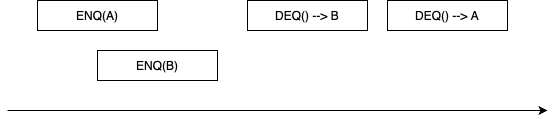
\includegraphics[scale=0.5]{pics/good}
  \caption{\label{fig::goodexample}An example of a linearizable execution. Either \texttt{Enqueue(A)} or \texttt{Enqueue(B)} could take effect first since they are concurrent.}
\end{figure}

\begin{figure}[hbt]
  \center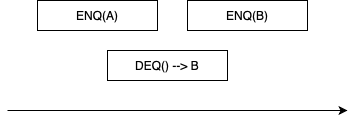
\includegraphics[scale=0.5]{pics/bad}
  \caption{\label{fig::badexample}An example of an execution that is not linearizable. Since \texttt{Enqueue(A)} has completed before \texttt{Enqueue(B)} is invoked the \texttt{Dequeue()} should return \texttt{A} or nothing.}
\end{figure}


There are various progress properties; the strongest is wait-freedom, and the more common is lock-freedom. An algorithm is \textit{wait-free} if each operation terminates after a finite number of its own steps. We call an algorithm \textit{lock-free} if, after a sufficient number of steps, one operation terminates. A wait-free algorithm is also lock-free but not vice versa; in an infinite run of a lock-free algorithm there might be an operation that takes infinitely many steps but never terminates.

In section 2 we talk about previous queues and their common problems. We also talk about polylogarithmic construction of shared objects.

Jayanti~\cite{DBLP:conf/podc/Jayanti98a} proved an $\Omega(\log p)$ lower bound on the worst-case shared-access time complexity of $p$-process universal constructions. He also introduced~\cite{DBLP:conf/podc/ChandraJT98} a construction that achieves $\textsc{O}(\log^2 p)$ shared accesses. Here, we first introduce a universal construction using $\textsc{O}(\log p)$ CAS operations~\cite{DBLP:conf/fsttcs/JayantiP05}. In section 3 we introduce a polylogarithmic step wait-free universal construction. Our main ideas in of the universal construction also appear in our Queue Algorithm (\ref{algQ}). The main short come of our universal construction is using big CAS objects. We use the universal construction as a stepping stone towards our queue algorithm, so we will not explain it in too much detail.

In section 4 we introduce a concurrent wait-free datastructure, to agree on the order of the operations invoked on some processes.

In section 5 we introduce our main work, the queue; prove its linearizability and wait-freeness.

\section{Related Work}
\subsection{List-based Queues}
In the following paragraphs, we look at previous lock-free queues.
Michael and Scott~\cite{DBLP:conf/podc/MichaelS96} introduced a lock-free queue which we refer to as the MS-queue. A version of it is included in the standard Java Concurrency Package. Their idea is to store the queue elements in a singly-linked list (see Figure~\ref{fig::msq}). Head points to the first node in the linked list that has not been dequeued, and Tail points to the last element in the queue. To insert a node into the linked list, they use atomic primitive operations like \texttt{LL/SC} or \texttt{CAS}. If $p$ processes try to enqueue simultaneously, only one can succeed, and the others have to retry. This makes the amortized number of steps to be $\Omega(p)$ per enqueue. Similarly, dequeue can take $\Omega(p)$ steps.

\begin{figure}[hbt]
  \center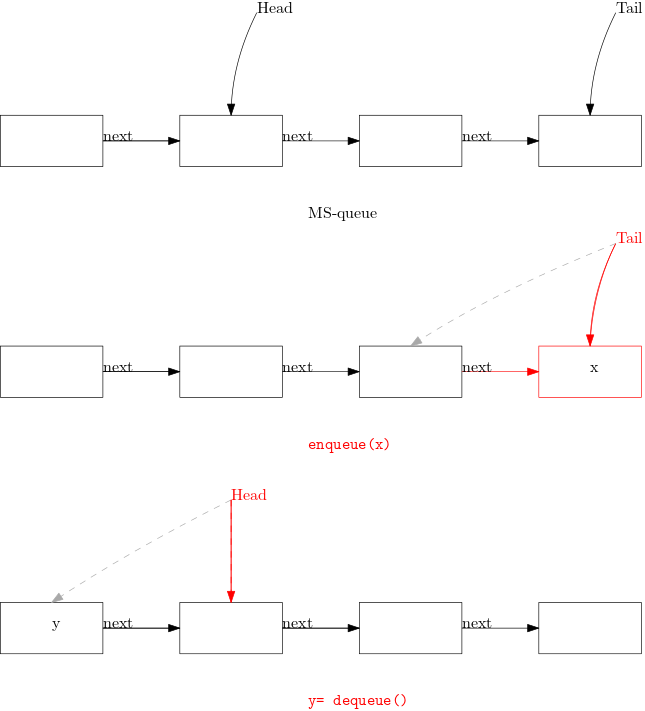
\includegraphics[scale=0.4]{pics/msqueue}
  \caption{\label{fig::msq}MS-queue structure, enqueue and dequeue operations. In the first diagram the first element has been dequeued. Red arrows show new pointers and gray dashed arrows show the old pointers.}
\end{figure}


Moir, Nussbaum, and Shalev~\cite{DBLP:conf/spaa/MoirNSS05} presented a more sophisticated queue by using the elimination technique. The elimination mechanism has the dual purpose of allowing operations to complete in parallel and reducing contention for the queue. An Elimination Queue consists of an MS-queue augmented with an elimination array. Elimination works by allowing opposing pairs of concurrent operations such as an enqueue and a dequeue to exchange values when the queue is empty or when concurrent operations can be linearized to empty the queue. Their algorithm makes it possible for long-running operations to eliminate an opposing operation. The empirical evaluation showed the throughput of their work is better than the MS-queue, but the worst case is still the same; in case there are $p$ concurrent enqueues, their algorithm is not better than MS-queue. 

Hoffman, Shalev, and Shavit~\cite{DBLP:conf/opodis/HoffmanSS07} tried to make the MS-queue more parallel by introducing the Baskets Queue. Their idea is to allow more parallelism by treating the simultaneous enqueue operations as a basket. Each basket has a time interval in which all its nodes' enqueue operations overlap. Since the operations in a basket are concurrent, we can order them in any way. Enqueues in a basket try to find their order in the basket one by one by using \texttt{CAS} operations. However, like the previous algorithms, if there are still $p$ concurrent enqueue operations in a basket, the amortized step complexity remains $\Omega(p)$ per operation.

\begin{figure}[hbt]
  \center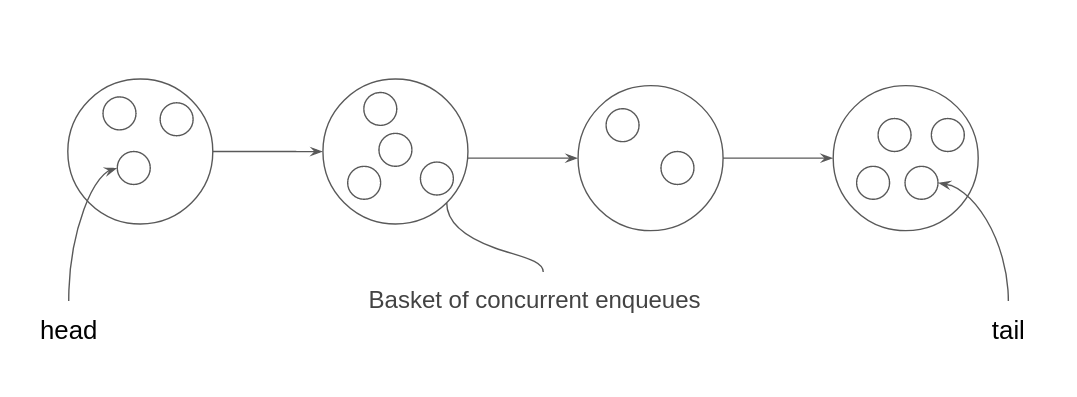
\includegraphics[scale=0.3]{pics/baskets}
  \caption{Baskets queue idea. There is a time that all operations in a basket were running concurrently, but only one has succeeded to do \texttt{CAS}. To order the operations in a basket, the mechanism in the algorithm for processes is to \texttt{CAS} again. The successful process will be the next one in the basket and so on.}
\end{figure}

Ladan-Mozes and Shavit~\cite{DBLP:journals/dc/Ladan-MozesS08} presented an Optimistic Approach to Lock-Free FIFO Queues. They use a doubly-linked list and do fewer \texttt{CAS} operations than MS-queue. But as before, the worst case is when there are $p$ concurrent enqueues which have to be enqueued one by one. The amortized worst-case complexity is still $\Omega(p)$ \texttt{CAS}es.

Hendler et al.~\cite{DBLP:conf/spaa/HendlerIST10} proposed a new paradigm called flat combining. Their queue is linearizable but not lock-free. Their main idea is that with knowledge of all the history of operations, it might be possible to answer queries faster than doing them one by one. In our work we also maintain the whole history. They present experiments that show their algorithm performs well in some situations.

Gidenstam, Sundell, and Tsigas~\cite{DBLP:conf/opodis/GidenstamST10} introduced a new algorithm using a linked list of arrays. Global head and tail pointers point to arrays containing the first and last elements in the queue. Global pointers are up to date, but head and tail pointers may be behind in time. An enqueue or a dequeue searches in the head array or tail array to find the first unmarked element or last written element (see~Figure~\ref{fig::sundell}). Their data structure is lock-free. Still, if the head array is empty and $p$ processes try to enqueue simultaneously, the step complexity remains $\Omega(p)$.

\begin{figure}[hbt]
  \center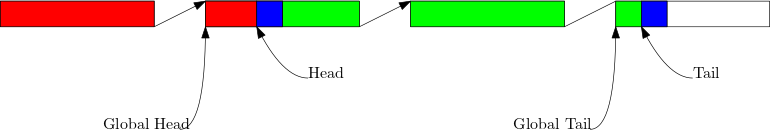
\includegraphics[scale=0.5]{pics/sundell}
    \caption{\label{fig::sundell}Global pointers point to arrays. Head and Tail elements are blue, dequeued elements are red and current elements of the queue are green.}
\end{figure}

Kogan and Petrank~\cite{DBLP:conf/ppopp/KoganP11} introduced wait-free queues based on the MS-queue and use Herlihy's helping technique to achieve wait-freedom. Their step complexity is $\Omega(p)$ because of the helping mechanism.

%todo: comparison
%Milman et al.~\cite{DBLP:conf/spaa/MilmanKLLP18} designed BQ: A Lock-Free Queue with Batching. Their idea of batching allows a sequence of operations to be submitted as a batch for later execution. It supports a new notion introduced by the authors called Extended Medium Futures Linearizability.

%Nikolaev and Ravindran~\cite{DBLP:journals/corr/abs-2201-02179} wCQ to be completed.
In the worst-case step complexity of all the list-based queues discussed above, there is a $p$ term that comes from the case all $p$ processes try to do an enqueue simultaneously. Morrison and Afek call this the \textit{CAS retry problem}~\cite{DBLP:conf/ppopp/MorrisonA13}. It is not limited to list-based queues and array-based queues share the CAS retry problem as well~\cite{DBLP:conf/spaa/TsigasZ01,DBLP:conf/icdcn/Shafiei09,DBLP:conf/iceccs/ColvinG05} . We are focusing on seeing if we can implement a queue in sublinear steps in terms of $p$ or not.

\subsection{Universal Constructions}
Herlihy discussed the possibility of implementing shared objects from other objects~\cite{10.1145/114005.102808}. A \textit{universal construction} is an algorithm that can implement a shared version of any given sequential object. We can implement a concurrent queue using a universal construction. Jayanti proved an $\Omega(\log p)$ lower bound on the worst-case shared-access time complexity of $p$-process universal constructions~\cite{DBLP:conf/podc/Jayanti98a}. He also introduced a construction that achieves $\textsc{O}(\log^2 p)$ shared accesses~\cite{DBLP:conf/podc/ChandraJT98}. His universal construction can be used to create any data structure, but its implementation is not practical because of using unreasonably large-sized \texttt{CAS} operations.

Ellen and Woelfel introduced an implementation of a Fetch\&Inc object with step complexity of $O(\log p)$ using $O(\log n$)-bit \texttt{LL/SC} objects, where $n$ is the number of operations~\cite{10.1007/978-3-642-41527-2_20}. Their idea has similarities to Jayanti's construction, and they represent the value of the Fetch\&Inc using the history of successful operations. 

%FIFO queues have a wide range of use in OS and applications. The current state-of-the-art queues are implemented using linked lists; that's why they have factor p in their time complexity.

%\href{https://docs.google.com/spreadsheets/d/1cL1tgXXdljkh462sMwkTVMHH_k0MBTmslIVM3xA5VS4/edit#gid=0}{Table of previous works}

%There is a connection between queues and universal constructions. We can implement a universal construction using a queue. We can store operations in the shared queue and compute operations' responses using the queue's content. Some impractical universal constructions are using big words as "...".

\pagebreak
\section{ Universal Construction using Tournament Tree with Big CAS Objects }

\paragraph{}
A universal construction gets any sequential object and creates a concurrent version of the given datastructure. Our universal construction in Algorithm~\ref{alg1} relies on a tournament tree with $p$ leaves and height $\log(p)$ is shared among $p$ processes. Nodes in the tree are CAS objects that store an ordering and support \tt{append()} and \tt{diff()} operations. Leaf $l_i$ stores the sequence of the operations invoked by $P_i$. Each internal node stores the sequence of operations propagated up to it. When process $P_i$ wishes to apply an operation $op$ on the implemented object, it appends $op$ to its assigned leaf and tries to propagate it up to the root. The history of operations stored at the root is the linearization ordering. The operation $op$ is linearized when it is appended to the root.

\begin{center}
\Tree [ [ [ $P_1$ $P_2$ ] [ $P_3$ $P_4$ ] ]
          [ [ $P_5$ $P_6$ ] [ $P_7$ $P_8$ ] ] ]
\end{center}


The algorithm uses a subroutine \textsc{Refresh}($n$) that concatenates new operations from node $n$'s children (that have not already been propagated to $n$) to the sequence of operations stored in $n$ and tries to CAS the new sequence into $n$. In other words, \textsc{Refresh}($n$) tries to append $n$'s children's new operations to $n$'s sequence.
After a process adding a new operations to its leaf, it has to propagate new operations up to the root. \textsc{Propagate}($n$) tries to append $n$'s new operations to the root $n$ by recursively calling \textsc{Refresh}($n$). In each \tt{Propagate()} step if a \textsc{Refresh}($n$) fails, it means another CAS operation has succeeded; if so, it tries to \textsc{Refresh}($n$) again. If the second attempt fails too, another process has already appended the operations the current \textsc{Propagate} is trying to append.
Operations that were in $l_i$ before \textsc{Propagate}($l_i$.parent) was invoked are guaranteed to be added to the root by the time the \textsc{Propagate}($l_i$.parent) terminates.



\begin{figure}
\begin{center}
\begin{subfigure}[b]{.49\textwidth}
  \centering
  \resizebox{\columnwidth}{!}{
  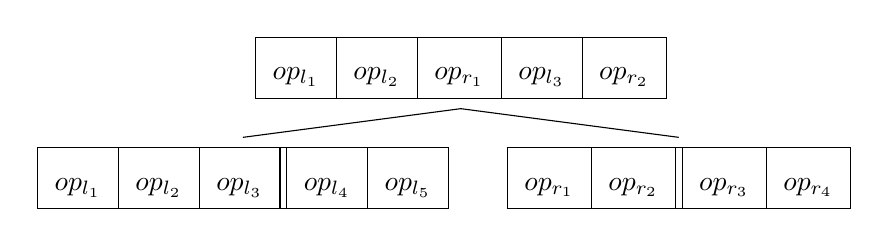
\begin{tikzpicture}[level 1/.style={level distance=1.4cm,sibling distance=0.5cm}]
\Tree [.{\begin{tabular}{|c|c|c|c|c|c|}  \hline $op_{l_1}$ & $op_{l_2}$ & $op_{r_1}$ & $op_{l_3}$ & $op_{r_2}$ \\ \hline \end{tabular}}
{\begin{tabular}{|c|c|c||c|c|}  \hline $op_{l_1}$ & $op_{l_2}$ & $op_{l_3}$ & $op_{l_4}$ & $op_{l_5}$ \\ \hline \end{tabular}}
{\begin{tabular}{|c|c||c|c|}  \hline $op_{r_1}$ & $op_{r_2}$ & $op_{r_3}$ & $op_{r_4}$\\ \hline \end{tabular}} ]
\end{tikzpicture}
}
  \caption{Operations after $||$ are new.}

\end{subfigure}
\hfill
\begin{subfigure}[b]{.49\textwidth}


  \centering
  \resizebox{\columnwidth}{!}{
  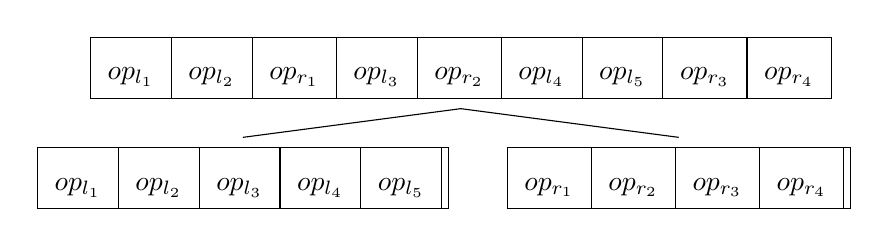
\begin{tikzpicture}[level 1/.style={level distance=1.4cm,sibling distance=0.5cm}]
\Tree [.{\begin{tabular}{|c|c|c|c|c|c|c|c|c|c|}  \hline $op_{l_1}$ & $op_{l_2}$ & $op_{r_1}$ & $op_{l_3}$ & $op_{r_2}$ & $op_{l_4}$ & $op_{l_5}$ & $op_{r_3}$ & $op_{r_4}$  \\ \hline \end{tabular}}
{\begin{tabular}{|c|c|c|c|c||}  \hline $op_{l_1}$ & $op_{l_2}$ & $op_{l_3}$ & $op_{l_4}$ & $op_{l_5}$ \\ \hline \end{tabular}}
{\begin{tabular}{|c|c|c|c||}  \hline $op_{r_1}$ & $op_{r_2}$ & $op_{r_3}$ & $op_{r_4}$\\ \hline \end{tabular}} ]
\end{tikzpicture}
}
  \caption{New operations are added to the parent node.}

\end{subfigure}


\caption{\label{fig:ucexample} Propagate Step in Universal Construction}
\end{center}
\end{figure}


\begin{algorithm}
\caption{Universal Construction Idea}\label{alg1}
\begin{algorithmic}[1]
\begin{multicols}{2}

\Function{response}{Do}{\textsl{operation} op, \textsl{pid} i} 
\State \texttt{l\textsubscript{i}.\Call{append}{op}}
\State \Call{Propagate}{parent of l\textsubscript{i}}
\State \texttt{Run} \textsf{the sequence stored in root}
\State \texttt{\Return op}\textsf{'s response from line 4}
\EndFunction{Do}

\Statex

\Function{void}{Propagate}{\textsl{node} n}
\If{\texttt{n==root}} \Return
\ElsIf{!\Call{Refresh}{n}}
\State \Call{Refresh}{$n$} \EndIf
\State \Call{Propagate}{parent of n}
\EndFunction{Propagate}

\columnbreak

\Function{boolean}{Refresh}{\textsl{node} n}
\State \texttt{old=} \Call{Read}{n}
\State \texttt{new=} \textsf{ops that n's children contain but \texttt{old} does not}
\State \texttt{new= old$\cdot$new}
\State \Return n.\Call{CAS}{old, new}
\EndFunction{Refresh}

\end{multicols}
\end{algorithmic}
\end{algorithm}


$\textsc{O}(\log n)$ CAS operations are invoked to do a \textsc{Propagate}, but the CAS words store sequences of unbounded length.
The problem is that we are trying to store unbounded sequence of operations in each node $n$ (see Figure~\ref{fig::uc}). However, to compute the result of an operation, we only use the total ordering that is stored at the root. Although we use a similar construction for our queue implementation, we develop an implicit representation of the sequence of operations, so that we can use reasonable sized CAS objects and still achieve polygarithmic step complexity.

\begin{figure}[h]
\begin{center}
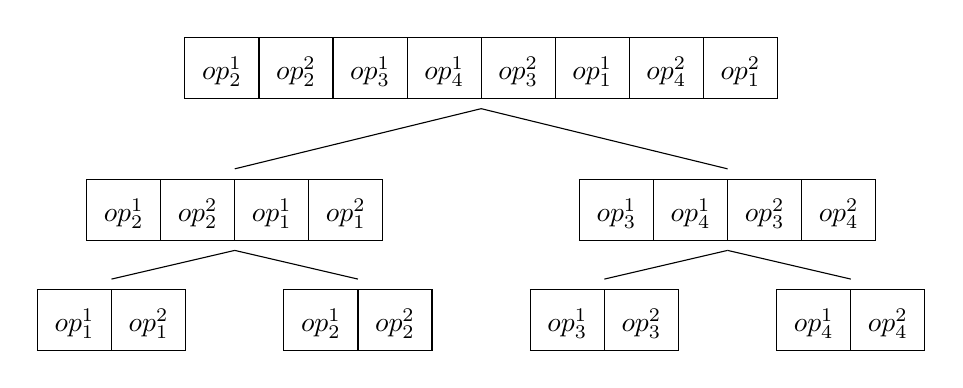
\begin{tikzpicture}[level 1/.style={level distance=1.8cm,sibling distance=1cm}, level 2/.style={level distance=1.4cm,sibling distance=1cm}]
  
\Tree [.{\begin{tabular}{|c|c|c|c|c|c|c|c|c|c}  \hline  $op_2^1$ & $op_2^2$ & $op_3^1$ & $op_4^1$ & $op_3^2$ & $op_1^1$ & $op_4^2$ & $op_1^2$ \\ \hline\end{tabular}}  [.{\begin{tabular}{|c|c|c|c|c|c}  \hline $op_2^1$ & $op_2^2$ & $op_1^1$ & $op_1^2$ \\ \hline\end{tabular}}
      {\begin{tabular}{|c|c|c|c}  \hline $op_1^1$ & $op_1^2$ \\ \hline\end{tabular}} {\begin{tabular}{|c|c|c|c}  \hline $op_2^1$ & $op_2^2$ \\ \hline\end{tabular}} ] [.{\begin{tabular}{|c|c|c|c|c|c}  \hline $op_3^1$ & $op_4^1$ & $op_3^2$ & $op_4^2$ \\ \hline\end{tabular}} {\begin{tabular}{|c|c|c|c}  \hline $op_3^1$ & $op_3^2$ \\ \hline\end{tabular}} {\begin{tabular}{|c|c|c|c}  \hline $op_4^1$ & $op_4^2$ \\ \hline\end{tabular}} ] ]

\end{tikzpicture}
\caption{\label{fig::uc} Universal Construction: $op_j^i$ denotes the $i$th operation from process $j$. In each node, we store the ordering of all the operations propagated up to it.}
\end{center}
\end{figure}



\pagebreak
\section{Block Trees}
Here we introduce a data structure that allows processes to agree on the linearization ordering of their operations using $\textsc{O}(\log p)$ \texttt{CAS} per operation called a \textit{block tree}. Then we use the block tree as a stepping stone towards our queue algorithm.
A block tree is a tournament tree shared among $p$ processes (see Figure~\ref{fig::blocktree}). Each process has a leaf, and it appends its operations to its leaf. After that, the process tries to propagate its new operation up to the tree's root. An ordering of operations propagated up to a node is stored in that node. All processes agree on the sequence stored in the root and this is used as the linearization ordering. Our idea is similar to Jayanti and Petrovic's multi-enqueuer single-dequeuer Queue~\cite{DBLP:conf/fsttcs/JayantiP05}, but we do not use \texttt{CAS} operations with big words and do not put a limit on the number of concurrent operations.

\begin{figure}[hbt]
\begin{center}
\Tree [ [ [ $P_1$ $P_2$ ] [ $P_3$ $P_4$ ] ]
          [ [ $P_5$ $P_6$ ] [ $P_7$ $P_8$ ] ] ]
\end{center}
\caption{ّ\label{fig::blocktree}In the block tree each process has a leaf and in each node there is an ordering of operations stored. Each node tries to propagate its operations up to the root, which stores the final ordering of all operations.}  
\end{figure}

The goal here is to ensure that in each propagate step the new operations are propagated up to the parent in $O(\log p)$ steps (see~Figure~\ref{fig::propagstep}). Then, a dequeue operation uses the linearization ordering to compute its answer.


In each propagate step, our algorithm uses a subroutine \textsc{Refresh}($n$) that aggregates new operations from node $n$'s children (that have not already been propagated to $n$) and tries to append them into $n$ using a \texttt{CAS} operation. The general idea is that if we call \textsc{Refresh}($n$) twice, the operations in $n$'s children before the first \textsc{Refresh}($n$) are guaranteed to be in $n$.
%Since there is a successful instance of \textsc{Refresh}($n$) after the first \textsc{Refresh}($n$), which has appended the talked operations.
Instead of storing operations explicitly in the nodes, we only keep track of the number of them. This allows us to \texttt{CAS} fixed-size objects in each \textsc{Refresh}($n$). To do that, we introduce blocks that only contain the number of operations from the left and the right child in a \texttt{Refresh}() procedure and only propagate the block of the new operations.
\pagebreak

\begin{figure}[hbt]
\begin{center}
\begin{subfigure}[b]{.49\textwidth}
  \centering
  \resizebox{\columnwidth}{!}{
  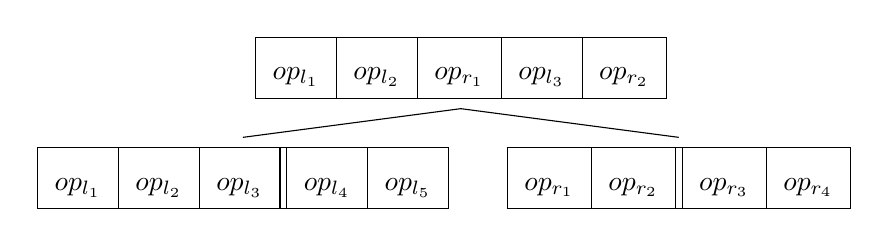
\begin{tikzpicture}[level 1/.style={level distance=1.4cm,sibling distance=0.5cm}]
\Tree [.{\begin{tabular}{|c|c|c|c|c|c|}  \hline $op_{l_1}$ & $op_{l_2}$ & $op_{r_1}$ & $op_{l_3}$ & $op_{r_2}$ \\ \hline \end{tabular}}
{\begin{tabular}{|c|c|c||c|c|}  \hline $op_{l_1}$ & $op_{l_2}$ & $op_{l_3}$ & $op_{l_4}$ & $op_{l_5}$ \\ \hline \end{tabular}}
{\begin{tabular}{|c|c||c|c|}  \hline $op_{r_1}$ & $op_{r_2}$ & $op_{r_3}$ & $op_{r_4}$\\ \hline \end{tabular}} ]
\end{tikzpicture}}
  \caption{Operations after $||$ are new.}
\end{subfigure}
\hfill
\begin{subfigure}[b]{.49\textwidth}
  \centering
  \resizebox{\columnwidth}{!}{
  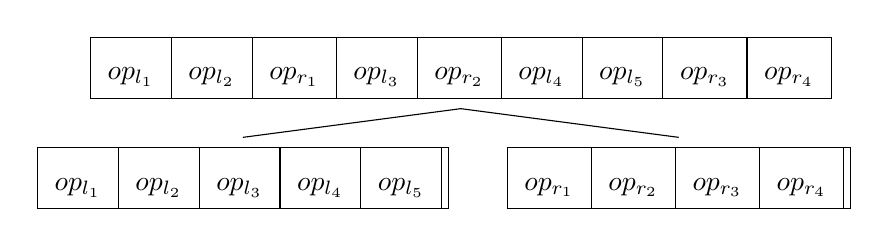
\begin{tikzpicture}[level 1/.style={level distance=1.4cm,sibling distance=0.5cm}]
\Tree [.{\begin{tabular}{|c|c|c|c|c|c|c|c|c|c|}  \hline $op_{l_1}$ & $op_{l_2}$ & $op_{r_1}$ & $op_{l_3}$ & $op_{r_2}$ & $op_{l_4}$ & $op_{l_5}$ & $op_{r_3}$ & $op_{r_4}$  \\ \hline \end{tabular}}
{\begin{tabular}{|c|c|c|c|c||}  \hline $op_{l_1}$ & $op_{l_2}$ & $op_{l_3}$ & $op_{l_4}$ & $op_{l_5}$ \\ \hline \end{tabular}}
{\begin{tabular}{|c|c|c|c||}  \hline $op_{r_1}$ & $op_{r_2}$ & $op_{r_3}$ & $op_{r_4}$\\ \hline \end{tabular}} ]
\end{tikzpicture}}
  \caption{New operations are added to the parent node.}
\end{subfigure}
\caption{\label{fig::propagstep} Successful \texttt{Refresh}, operations in children after $||$ are new.}
\end{center}
\end{figure}

We also implement methods \texttt{Get(i)}, \texttt{Index(op)} to get the $i$th propagated operation and compute the rank of a propagated operation in the linearization. \texttt{Get(i)} finds the block containing the $i$th operation in the root and then finds its sub-block recursively to reach a leaf. \texttt{Index()} is  similar but more complicated, finding super-blocks from a leaf to the root. The main challenge in each level of \texttt{Get(i)} and \texttt{Index(op)} is that it should take polylogarithmic steps with respect to $p$. After appending operation \texttt{op} to the root, processes can find out information about the linearization ordering using \texttt{Get(i)} and \texttt{Index(op)}. 

\texttt{Get()} and \texttt{Index()} search among blocks in each level of the tree to find the sub-block or super-block containing the given operation. Each block stores a constant amount of information (like prefix sums) to allow binary searches to find the required block in a node quickly.

Block tree can be used to implement queue, but \texttt{Get(i)}  may take a long time since it has to find the block containing the $i$th operation at the root level.



%\subsection{Idea in a nutshell}
We apply two ideas from universal construction to create a new linearizable data structure agreeing on a sequence of elements among processes. First, there is a shared tournament tree among processes, in which each process appends its element to its leaf in the tree and then tries to propagate it up to the root by performing \textsc{Refresh()} operations at each node. Second, each operation is linearized when its element is appended to the root.



\paragraph{}
 In the universal construction, we order new concurrent operations at each \textsc{Refresh}() and maintain that order in the path up to the root. However, we can instead keep track of sets of concurrent operations and create the total ordering of all operations at the root (see Figure~\ref{fig::set}).
 
 \begin{figure}[h]
\begin{center}
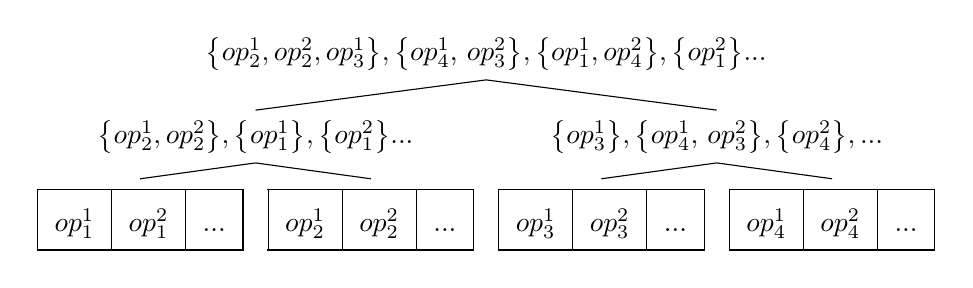
\begin{tikzpicture}
  
\Tree [.{$\big\{op_2^1,op_2^2,op_3^1\big\},\big\{op_4^1$, $op_3^2\big\},\big\{op_1^1, op_4^2\big\},\big\{op_1^2\big\}...$ }  [.{ $\big\{op_2^1, op_2^2\big\},\big\{op_1^1\big\},\big\{op_1^2\big\}...$ }
      {\begin{tabular}{|l|c|c|c}  \hline $op_1^1$ & $op_1^2$ & ... \\ \hline\end{tabular}} {\begin{tabular}{|l|c|c|c}  \hline $op_2^1$ & $op_2^2$ & ... \\ \hline\end{tabular}} ] [.{ $\big\{op_3^1\big\},\big\{op_4^1$, $op_3^2\big\},\big\{op_4^2\big\},...$ } {\begin{tabular}{|l|c|c|c}  \hline $op_3^1$ & $op_3^2$ & ... \\ \hline\end{tabular}} {\begin{tabular}{|l|c|c|c} \hline $op_4^1$ & $op_4^2$ & ... \\ \hline\end{tabular}} ] ]

\end{tikzpicture}
\caption{\label{fig::set} In each internal node, we store the set of all the operations propagated together, and one can arbitrarily linearize the sets of concurrent operations among themselves. Since we linearize operations when they are added to the root, ordering the blocks in the root is important.}
\end{center}
\end{figure}


The definition of linearizability allows concurrent operations to be reordered arbitrarily. Thus, a group of concurrent operations can be appended to our root sequence as one block without specifying the order among the operations.


%\begin{lemma}
%Operations in the same block can be linearized in any order.
%\end{lemma}


\paragraph{}
 We used unbounded CAS objects storing sequences as big words in the universal construction. One can represent sequences as arrays to overcome this implementation problem. Each array element will store one of the blocks of concurrent operations described in section \ref{subsec::block}.
 


\paragraph{}
Copying operation sequences from children to their parent in a \textsc{Refresh}() takes time proportioned to the number of operations being copied. This is time-consuming, so we propose a way to augment the tree to calculate lines 15,16 in $\textsc{O}(\log p)$ steps which reads new operation and concats them with old operations. Instead of representing the set of operations by explicitly listing them in a node, we represent a set of operations implicitly by recording which of the children's sets were unioned to create the set. Having operation sequences stored at leaves, we can deduce a set of operations in a node using this implicit representation.~(see Figure~\ref{fig:block}.)

\pagebreak
\begin{figure}

\begin{center}
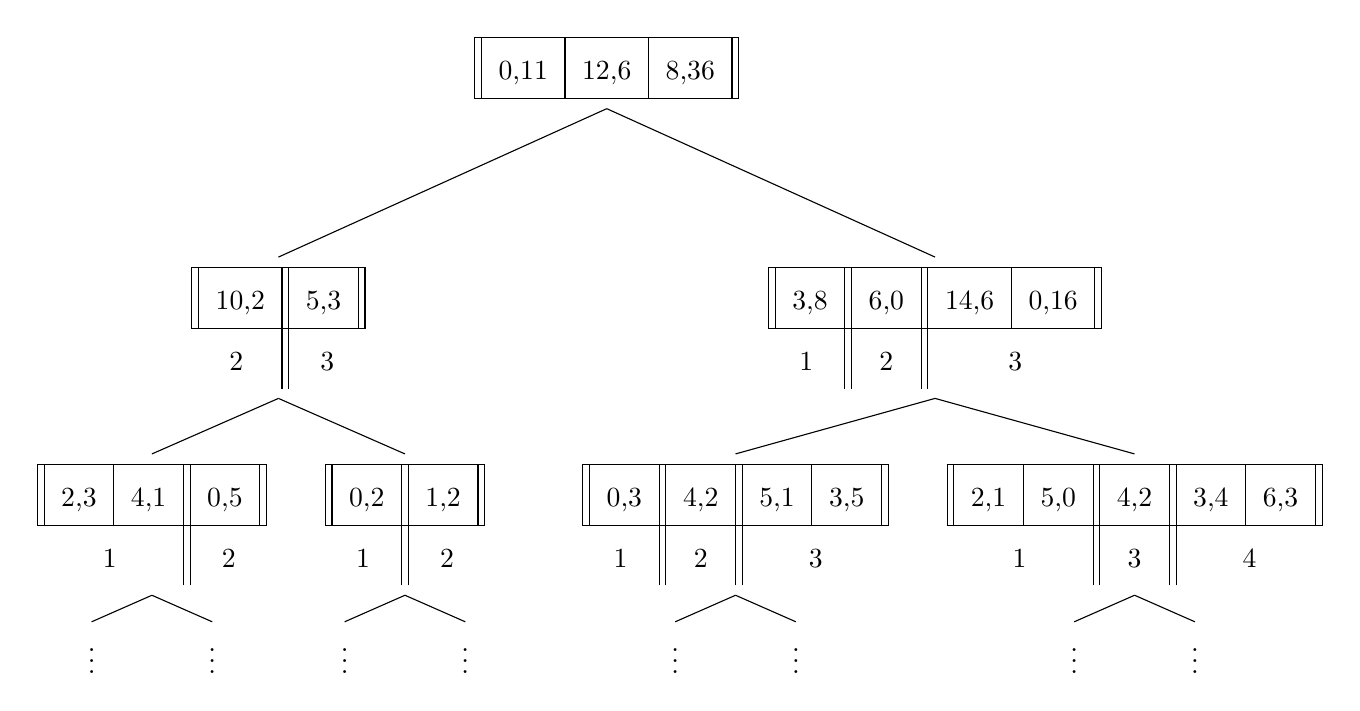
\begin{tikzpicture}[level 1/.style={level distance=3.3cm,sibling distance=1cm},
	level 2/.style={level distance=2.5cm,sibling distance=0.5cm},
	level 3/.style={level distance=1.8cm,sibling distance=1.2cm}]
  

\Tree [.{\begin{tabular}{||c|c|c||}  \hline 0,11 & 12,6 & 8,36 \\ \hline\end{tabular}}
 [.{\begin{tabular}{||c||c||}  \hline 10,2 & 5,3 \\  \hline \multicolumn{1}{c||}{2} & \multicolumn{1}{c}{3} \end{tabular}}
 [.{\begin{tabular}{||c|c||c||}\hline 2,3 & 4,1 & 0,5 \\\hline\multicolumn{2}{c||}{1} & \multicolumn{1}{c}{2}\end{tabular}} $\vdots$ $\vdots$ ]
  [.{\begin{tabular}{||c||c||}  \hline 0,2 & 1,2 \\  \hline \multicolumn{1}{c||}{1} & \multicolumn{1}{c}{2} \end{tabular}} $\vdots$ $\vdots$ ] ]
          [.{\begin{tabular}{||c||c||c|c||}  \hline 3,8 & 6,0 & 14,6 & 0,16 \\ \hline \multicolumn{1}{c||}{1} & \multicolumn{1}{c||}{2} & \multicolumn{2}{c}{3}\end{tabular}}
           [.{\begin{tabular}{||c||c||c|c||}  \hline 0,3 & 4,2 & 5,1 & 3,5 \\ \hline \multicolumn{1}{c||}{1} & \multicolumn{1}{c||}{2}& \multicolumn{2}{c}{3}\end{tabular}} $\vdots$ $\vdots$ ]
            [.{\begin{tabular}{||c|c||c||c|c||}  \hline 2,1 & 5,0 & 4,2 & 3,4 & 6,3 \\ \hline \multicolumn{2}{c||}{1} & \multicolumn{1}{c||}{3} & \multicolumn{2}{c}{4}\end{tabular}} $\vdots$ $\vdots$ ] ] ]

\end{tikzpicture}
\end{center}
\caption{\label{fig:block} Showing concurrent operation sets with blocks. Each block consists of a pair(left, right) indicating the number of operations from the left and the right child, respectively. Block (12,6) in the root contains blocks (10,2) from the left child and (6,0) from the right child. Blocks between two lines $||$ are propagated together to the parent. For example, Blocks (2,3) and (4,1) from the leftmost leaf and (0,2) from its sibling are propagated together into the block (10,2) in their parent. The number underneath a group of blocks in a node indicates which block in the node's parent those blocks were propagated to.}
\end{figure}


Each block $b$ in node $n$ is the aggregation of blocks in the  children of $n$ that are newly read by the\textsc{Propagate}() step that created block $b$. For example, the third block in the root (8,36) is created by merging block (5,3) from the left child and (14,6) and (0,16) from the right child. Block (5,3) also points to elements from blocks (0,5) and (1,2). 
%Recursively we can deduce each block contents until the leaf nodes store arrays of individual element operations.

\begin{definition}\{Existence of an operation in a block\}  Operation op exists in block b if it has propagated up to block b.
\end{definition}


\begin{definition}\{Subblock\}
  The blocks that are aggregated into block $b$ in a \textsc{Propagate}() step are called subblocks of $b$. Block $b_1$ is a subblock of $b_2$ if and only if $b_1$ is a block in node $v$ and in $b_2$ is a block in the parent of $v$ and $b_1$'s elements exits in $b_2$'s elements.
\end{definition}
%{\TODO: describe how blocks work with a good example how exactly it is done}

\paragraph{}
We choose to linearize operations in a block from the left child before those from the right child as a convention. Operations within a block of the root can be ordered in any way that is convenient. In effect, this means that if there are concurrent new blocks in a \textsc{Refresh}() step from several processes we linearize them in the order of their process ids. So for example  operations aggregated in block (10,2) are in the order (2,3),(4,1),(0,2). All blocks from the left child with come before the right child and the order of blocks of each child is preserved among themselves.
%\begin{lemma}
%\label{lem:block_size}
%There cannot be more than one operation from each process in a \textsc{Refresh}() invocation.
%\end{lemma}
%\begin{proof}
%  If so, then that parent process has invoked two simultaneous operations. $ \blacksquare $
%\end{proof}

\paragraph{}
In a \textsc{Propagate}() invocation path from a leaf to root, there will be \textsc{Refresh}() steps with merges from $2, 4, 8, ..., p$ processes. So in a complete propagation, at most $2p$ blocks are merged into one block. \texttt{(maybe useful for analysis)}
%\begin{lemma}
%A block in the root cannot contain more than one operation from a process.
%\end{lemma}
%\begin{proof}
%  Assume a process in a block invokes two operations; one has to be finished another. If so, it has been added to root before. $\blacksquare$
%\end{proof}

\pagebreak
\subsection{Using pointers and prefix sum to make \textsc{GetIndex}($i$) faster}
%\begin{definition}
%  \textsc{BSearch}($i$): Search $i$th element in a prefix sum array with length $n$ in \textsc{O}($\log n$) steps.
%\end{definition}
\paragraph{}
\textsc{GetIndex}($i$) returns the $i$th operation stored in the block tree sequence. We do that by finding the block $b_i$ containing $i$th element in the root, and then recursively finding the subblock of $b_i$ which contains $i$th element. To make this recursive search faster, instead of iterating over all elements in sequence of blocks we store prefix sum of number of elements in the blocks sequence and pointers to make BSearch faster.

Furthermore, in each block, we store the prefix sum of left and right elements. Moreover, for each block, we store two pointers to the last left and right subblock of it (see fig \ref{fig::pointer} and \ref{fig:prefix}).

\begin{figure}
\begin{center}
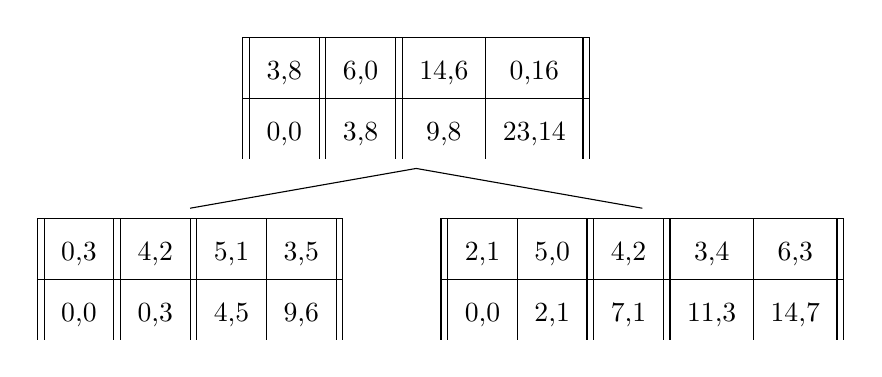
\begin{tikzpicture}[level 1/.style={level distance=2.3cm,sibling distance=1cm}]
  
\Tree [.{\begin{tabular}{||c||c||c|c||}  \hline 3,8 & 6,0 & 14,6 & 0,16 \\ \hline  0,0 & 3,8 & 9,8 & 23,14\end{tabular}}
           [.{\begin{tabular}{||c||c||c|c||}  \hline 0,3 & 4,2 & 5,1 & 3,5 \\ \hline 0,0 & 0,3 & 4,5 & 9,6 \end{tabular}} ]
            [.{\begin{tabular}{||c|c||c||c|c||}  \hline 2,1 & 5,0 & 4,2 & 3,4 & 6,3 \\ \hline 0,0 & 2,1 & 7,1 & 11,3 & 14,7 \end{tabular}} ] ]


\end{tikzpicture}
\end{center}
\caption{\label{fig:prefix} Using Prefix sums in blocks. When we want to find block b elements in its children, we can use binary search. The number below each block shows the count of elements in the previous blocks.}
\end{figure}

\begin{figure}[hbt]
\centering
  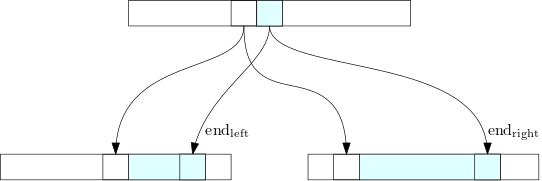
\includegraphics[width=5in]{pics/pointers}
  \caption{Block have pointers to the starting block of theirs for each child. \label{fig::pointer}}
\end{figure}

\paragraph{}
Starting from the root, \textsc{GetIndex}($i$) BSearches $i$ in the prefix sum array to find block containing $i$th operation, then continues recursively calling \textsc{GetElement}($b,i$) to find $i$th element of block $b$. From lemma $\ref{lem:block_size}$ we know a block size is at most $p$. So BSearch takes at most \textsc(O)$(\log p)$, since  with knowing pointers of a block and its previous block we can determine the base \texttt{(domain ?)} to search and its size is \textsc{O}$(p)$.


\pagebreak
\subsection{Block Tree Algorithm}
\paragraph{}
Our Block Tree is a linearizable implementation of a data structure that stores a sequence of elements. It has two methods (see Algorithm~\ref{alg2}), \textsc{Append}($e$) which appends element $e$ to the sequence, and \textsc{Get}($i$) which returns the $i$th element in the sequence.

\paragraph{Design of a block tree}

Each process is assigned to a leaf in a shared tournament tree. Thus, for example, the leaf node for process $p_i$ contains an array of elements by $p_i$ in the order they were invoked.
Each internal node of the tree contains an array of blocks of elements.
Block $b$ in node $n$ is created in a \textsc{Propagate}() step and is merged block of new blocks at the time of \textsc{Propagate}() reading $n$'s children blocks. Each block consists of pointers left and right, to the last block merged into itself from left and right child in that order. Moreover, two numbers, left and right, indicate the count of elements in the blocks from the left and right child consecutively. Furthermore, prefix left, and right can be computed from the prefix sum of left and right values.
Elements of block $b$ can be determined recursively (\textsc{GetElements($b$)}).
The $i$th element in the sequence can be determined in \textsc{O}($\log^2 p$) steps by recursively finding $i$th element in block $b$ (\textsc{GetElement($i$)})
After element $e$ is propagated (appended to a block int the root), its index can be computed with \textsc{GetIndex}($op$).


In order to compute elements of a block faster we store prefix-sum blocks(block i has tuple(right-sum=$\#$right ops in previous block, left-sum=$\#$left ops in previous blocks)[See Figure \ref{fig:prefix}]. Here is the algorithm to get elements of a block.

\paragraph{Specification}
A block tree is a shared data structure that stores a sequence of elements.  It has two methods \texttt{Append(e)} and \texttt{Get(i)}. \texttt{Append(e)} adds \texttt{e} to the end of the sequence and returns the index of \texttt{e} in the sequence. \texttt{Get(i)} returns \texttt{i}th element stored in the sequence. 

\paragraph{SubBlock} Block \texttt{s} is a subblock of \texttt{b} if \texttt{s} is between blocks \texttt{start..end} in \texttt{n} from Lines 41,42 of \texttt{CreateBlock()}.

\paragraph{Membership}
Element \texttt{e} is a member of block \texttt{b} in:
\begin{itemize}
  \item internal node \texttt{n}, if \texttt{e} is a memeber of \texttt{s} that \texttt{s} is a subblock of \texttt{b}.
  \item leaf node \texttt{n}, if \texttt{e} belongs to \texttt{n.dir.blocks[b\textsuperscript{$\prime$}.end\textsubscript{dir}+1..b.end\textsubscript{dir}]} for \texttt{dir} $\in$ \texttt{\{left, right\}} which b\textsuperscript{$\prime$} is the previous block of \texttt{b} in \texttt{n}.
\end{itemize}


\pagebreak
\paragraph{Order of elements inside node}
Element \texttt{d} is before element \texttt{e} in node \texttt{n}, if:
\begin{itemize}
  \item The block containing d is before the block containing e.
  \item e and d are in the same block and d is in the left child and e is in the right child.
  \item d is before e in the same child's order.
\end{itemize}


\begin{figure}[hbt]
  \center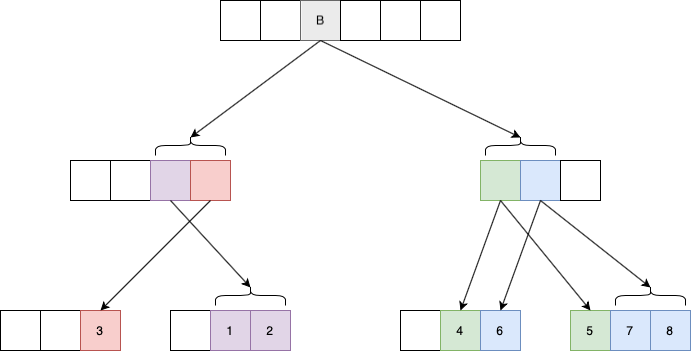
\includegraphics[width=5.5in]{pics/tree}
  \caption{Order of elements in b: elements in leaves are ordered with numerical order in the drawing.}
\end{figure}


\paragraph{\texttt{CreateBlock()}} \texttt{CreateBlock(n)} returns a block containing new operations of \texttt{n}'s children. \texttt{b\textsuperscript{$\prime$}.end\textsubscript{left}} stores the index of the rightmost subblock of left child of \texttt{b}'s previous block. Other attributes are assigned values followed by definition.
\begin{figure}[hbt]
  \center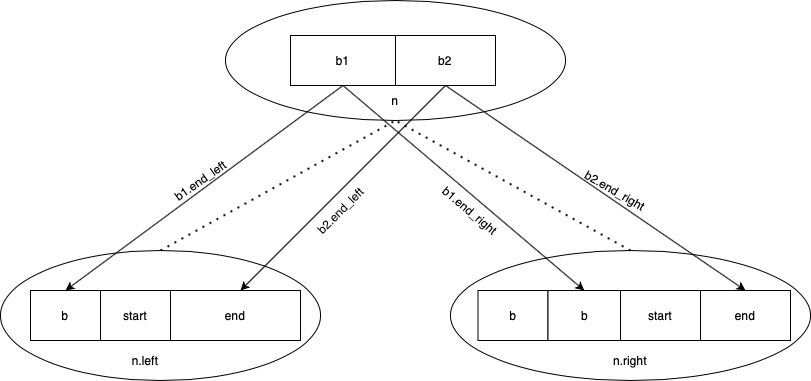
\includegraphics[width=5.5in]{pics/createblock}
  \caption{\label{fig::createBlock}Snapshot of a CreateBlock()}
\end{figure}

%\textsf{Is it necessary to say \texttt{CreateBlock()} is doing what it's supposed to do by definition? Or \texttt{Append()} for example?}


\pagebreak
\paragraph{Double Refresh}
Elements in \texttt{n}'s children's blocks before line \texttt{13} are guaranteed to be in \texttt{n}'s blocks after Line~\texttt{15}.
\begin{proof}
\texttt{CreateBlock()} reads blocks in the children that does not exist in the parent and aggregates them into one block. If a \texttt{Refresh} procedure returns true it means it has appended the block created by \texttt{CreateBlock()} into the parent node's sequence. So suppose two \texttt{Refresh}es fail. Since the first \texttt{Refresh} was not successful, it means another CAS operation by a \texttt{Refresh}, concurrent to the first\texttt{Refresh}, was successful before the second \texttt{Refresh}. So it means the second failed \texttt{Refresh} is concurrent with a successful \texttt{Refresh} that assuredly has read block before the mentioned line \texttt{13}. After all it means if any of the \texttt{Refresh} attempts were successful the claim is true, and also if both fail the mentioned claim still holds.
\end{proof}
\begin{figure}[hbt]
  \center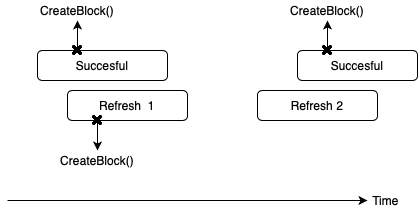
\includegraphics[width=4in]{pics/doublerefresh.png}
  \caption{The second failed Refresh is assuredly concurrent to a Successful \texttt{Refresh()} with \texttt{CreateBlock} line after first failed \texttt{Refresh}'s \texttt{CreateBlock()}.}
\end{figure}


\paragraph{Disjunction} Blocks in node \texttt{n}'s contain disjoint sets of elements.
\begin{proof}
Without loss of generality, assume blocks \texttt{b1, b2} contain common element \texttt{e} from the left child, and \texttt{b2} is after \texttt{b1} in \texttt{n}'s sequence of blocks. So block start of b2's \texttt{CreateBlock()} is after block end of \texttt{b1}'s end. Since \texttt{b2}'s start is the end of the block before itself, it cannot be before \texttt{b1}'s end.
\end{proof}

\paragraph{Total Order}
Sequence represented by the Block Tree is the sequence of the blocks stored in the root.

\paragraph{Linearization Points}
\texttt{Get(i)} is linearized when it terminates. \texttt{Append(e)} is linearized right after when a block containing \texttt{e} is appended to the root, if there are multiple elements appended together, they are linearized by the defined order in the root.

\paragraph{Subblocks Upperbound} Block b has at most $p$ subblocks.
\begin{proof}
If there are more than $p$ subblocks, then there is more than one block from process pl. \texttt{Append(e)} finishes after propagating and appending \texttt{e} to the root(line 9). So these blocks cannot be appended to root already, so pl has invoked two concurrent \texttt{Append()}s(line 1) without terminating the first one.
\end{proof}

\paragraph{Computing \texttt{Get(n, b, i)}}
To find the \texttt{i}th element in block \texttt{b} of node \texttt{n}, we search among subblocks of \texttt{b} that is bounded by $p$. Subblocks of a block are within the start and end block of the \texttt{CreateBlock()} procedure of it.

\paragraph{How \texttt{Refresh(n)} works.}
\begin{enumerate}
  \item Read n's counter and head
  \item Create block b
  \item CAS b into n
  \item If previous succeed:
  \begin{enumerate}
  \item Update sup of b's ending subblocks
  \item Increment children's counters
  \end{enumerate}
\end{enumerate}



\begin{figure}[hbt]
  \center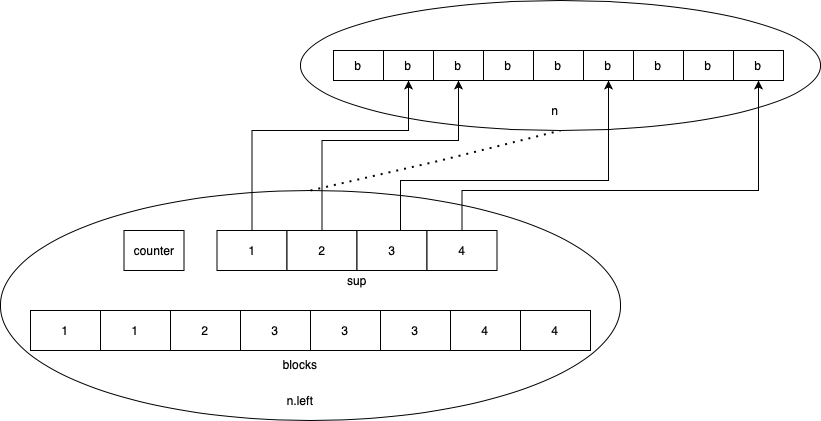
\includegraphics[width=6in]{pics/super}
  \caption{\texttt{Sup} and \texttt{timer} in a node, numbers on blocks are their \texttt{time} values.}
\end{figure}

\paragraph{Computing superblock}
\begin{enumerate}
  \item Value read for \texttt{super[b.time]} in line 71 is not null.\begin{proof}
    \texttt{Index()} is invoked after finishing \texttt{Propagate()} in line 10. For each value \texttt{c\textsubscript{dir}} read in lines 23, \texttt{super} is set before incrementing in lines 26,27.
  \end{proof} 
  \item \texttt{super[]} preserves order from child to parent; if in a child block \texttt{b} is before \texttt{c} then \texttt{b.time} $\leq$ \texttt{c.time} and \texttt{super[b.time]} $\leq$ \texttt{super[c.time]}\begin{proof}
   Follows from the order of lines 37, 26, 27.
 \end{proof}
%  \item In a propagate step at most 2 different time values are read \\ If there are more than 2 numbers then the smallest number should have been propagated far before.
%  \item There are at most $p^2$ blocks with same time value in a node. \\ At most p processes could die before line 27 and each contains at most p elements.
  \item \texttt{super[i+1]-super[i]}$\leq p$
\begin{proof}
 In a Refresh with successful CAS in line 24, \texttt{super} and \texttt{counter} are set for each child in lines 26,27. Assume the current value of the counter in node \texttt{n} is \texttt{i+1} and still \texttt{super[i+1]} is not set. If an instance of successful \texttt{Refresh(n)} finishes \texttt{super[i+1]} is set a new value and a block is added after \texttt{n.parent[sup[i]]}. There could be at most $p$ successful unfinished concurrent instances of \texttt{Refresh()} that have not reached line 27. So the distance between \texttt{super[i+1]} and \texttt{super[i]} is less than $p$.
 \end{proof}
  \item Superblock of \texttt{b} is within range $\pm 2p$ of the \texttt{super[b.time]}.
\begin{proof}
\texttt{super[i]} is the index of the superblock of a block containing block b. It is trivial to see that \texttt{n.super} and \texttt{n.b.counter} are increasing.  \texttt{super(b)} is the real superblock of b. \texttt{super(t]} is the index of the superblock of the last block with time \texttt{t}. If \texttt{b.time} is \texttt{t} we have:
$$super[t]-p\leq super[t-1]\leq super(t-1] \leq super(b) \leq super(t+1)\leq super(t+1]\leq super[t]+p$$
  \end{proof} 
\end{enumerate}



\section{Implementing Queue using Block Tree}
In this work, we design a queue with $O(\log^2 p +\log n)$ steps per operation, where $n$ is the number of total operations invoked. We avoid the $\Omega(p)$ worst-case step complexity of existing shared queues based on linked lists or arrays (CAS Retry Problem). A queue stores a sequence of elements and supports two operations, enqueue and dequeue. \texttt{Enqueue(e)} appends element \texttt{e} to the sequence stored.\texttt{Dequeue()} removes and returns the first element among in the sequence. If the queue is empty it returns \texttt{null}. Knowing index $i$ is the tail of the queue, we can return the dequeue response using \texttt{Get(i)}.  So in the rest we modify block tree to compute \texttt{i} for each \texttt{Dequeue()} to achieve a FIFO queue.
%
%\subsection{What should a \texttt{Dequeue()} return, regarding history of operations?}
\paragraph{}
Next, we describe how to use block tree to implement queues. The block tree, maintains the history of all operations, not only the current state of the queue. Now consider the following history of operations. What should each \texttt{Dequeue()} return? We can implement Enqueue and Dequeue using our block tree. An \texttt{Enqueue(e)} appends an operation with input argument \texttt{e} in the block tree. To do a \texttt{Dequeue()}, process $p$ first appends a \texttt{DEQ} operation to the tree. Then $p$ finds the rank of the \texttt{DEQ} using \texttt{Index()}, the rank of the \texttt{DEQ} and the information stored in the root about the queue $p$ computes the rank of  the \texttt{ENQ} having the answer of the \texttt{DEQ}. Finally $p$ returns the argument of that \texttt{ENQ} using \texttt{Get(i)}.

\begin{table}[hbt]
\centering
  \begin{tabular}{c|c|c|c|c|c|c|c|c|c}
    \hline \texttt{ENQ(5)}& \texttt{ENQ(2)}& \texttt{DEQ()}& \texttt{ENQ(3)}&\texttt{DEQ()}& \texttt{DEQ()}& \texttt{DEQ()}& \texttt{ENQ(4)}& \texttt{ENQ(6)}& \texttt{DEQ()}\\ \hline
  \end{tabular}
  \caption{An example histoy of operations on the queue}
\end{table}

\begin{definition}
A non-null dequeue is one that returns a non-null value.
\end{definition}

\paragraph{}
In the example above, \texttt{Dequeue()} operations return \texttt{5, 2, 3, null, 4} in order. Before \texttt{ENQ(4)} the queue gets empty so the last \texttt{DEQ()} returns null. If the queue is non-empty and $r$ \texttt{Dequeue()} operations have returned a non-null response, then $i$th \texttt{Dequeue()} returns the input of the $r+1$th \texttt{Enqueue()}. So, in order to answer a Dequeue, it's sufficent to know the size of the queue and the number of previous non-null dequeues.

%\texttt{DEQ[i] = (size>0) ? ENQ[r+1] : null;}


%\subsection{What should a \texttt{Dequeue()} return, regarding history of blocks of operations?}

\paragraph{}
In the Block Tree, we did not store the sequence of operations explicitly but instead stored blocks of concurrent operations to optimize \texttt{Propagate()} steps and increase parallelism. So now the problem is to find the result of each Dequeue. From lemma \ref{lem:block_size} we know we can linearize operations in a block in any order; here, we choose to decide to put Enqueue operations in a block before Dequeue operations. In the next example, operations in a cell are concurrent. \texttt{DEQ()} operations return \texttt{null, 5, 2, 1, 3, 4, null} respectively. We will next describe how these values can be computed efficiently.

\begin{table}[hbt]
\centering
  \begin{tabular}{c|c|c|c}
    \hline \texttt{DEQ()} & \texttt{ENQ(5)}, \texttt{ENQ(2)}, \texttt{ENQ(1)}, \texttt{DEQ()}& \texttt{ENQ(3)}, \texttt{DEQ()}&  \texttt{ENQ(4)}, \texttt{DEQ()}, \texttt{DEQ()}, \texttt{DEQ()}, \texttt{DEQ()}\\ \hline
  \end{tabular}
  \caption{An example history of operation blocks on the queue}
\end{table}

\pagebreak
\paragraph{}
Now, we claimed that by knowing the current size of the queue and the number of non-null dequeue operations before the current dequeue, we could compute the index of the resulting \texttt{Enqueue()}. We apply this approach to blocks; if we store the size of the queue after each block of operations happens and the number of non-null dequeues dequeues till a block, we can compute each dequeue's index of result in \textsc{O}$(1)$ steps.

\begin{table}[hbt]
\centering
  \begin{tabular}{c|c|c|c|c}
    \hline &\texttt{DEQ()} & \texttt{ENQ(5)}, \texttt{ENQ(2)}, \texttt{ENQ(1)}, \texttt{DEQ()}& \texttt{ENQ(3)}, \texttt{DEQ()}&  \texttt{ENQ(4)}, \texttt{DEQ()}, \texttt{DEQ()}, \texttt{DEQ()}, \texttt{DEQ()}\\ \hline
    \#enqueues & 0 & 3 & 1 & 1 \\ \hline
        \#dequeues & 1 & 1 & 1 & 4 \\ \hline
            \#non-null dequeues & 0 & 1 & 2 & 5 \\ \hline
                size & 0 & 2 & 2 & 0 \\ \hline
  \end{tabular}
  \caption{Augmented history of operation blocks on the queue}
\end{table}

%\begin{definition}
%  \texttt{index(op)}: index of the given Dequene among same type operation in conataing block.
%  
%  \texttt{INDEX(op)}: index of the given Dequene among same type operation in all operations.
%  
%\end{definition}

Size and the number of non-null dequeues for $b$th block could be computed this way:\\
\texttt{size[b]= max(size[b-1] +enqueues[b] -dequeues[b], 0)}\\
\texttt{non-null dequeues[b]= non-null dequeues[b-1] +dequeues[b] -size[b-1] -enqueues[b]}

Given \texttt{DEQ} is in block \texttt{b}, \texttt{response(DEQ)} would be:\\
\texttt{(size[b-1]- index of DEQ in the block's dequeus >=0) ? ENQ[non-null dequeus[b-1]+ index of DEQ in the block's dequeus] : null;}

\pagebreak
\section{Main Algorithm}

\paragraph{Specification}
A Queue is a shared data structure that stores a sequence of elements. It has two methods \texttt{Enqueue(e)} and \texttt{Dequeue()}. \texttt{Enqueue(e)} adds \texttt{e} to the end of the sequence. \texttt{Dequeue()} returns the first element stored in the sequence and removes it from the sequence.

\begin{figure}[hbt]
\centering
  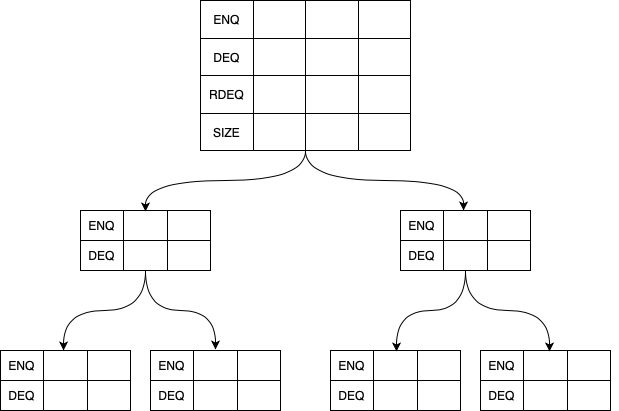
\includegraphics[width=5in]{pics/queue}
  \caption{Fields stored in the Queue nodes. \label{fig::queue}}
\end{figure}


\subsection{Pseudocode description}

\paragraph{Tournament Tree}
In order to reach an agreement on the order of operations among $p$ processes, we use a Tournament Tree. Leaf \texttt{l\textsubscript{i}} is assigned to a process \texttt{i}. Each process adds $op$ to its leaf. In each internal node an ordering of operations in its subtree is stored. All processes agree on the total ordering of all operations stored in the root. This ordering will be the linearization of the operations.
\paragraph{Implicit Storing Blocks}
For efficiency, instead of storing explicit sequence of operations in nodes of the Tournament Tree, we use Blocks. A Block is a constant size object that implicitly represents a sequence of operations. In each node there is an array of Blocks.

\begin{definition}[Block]
A block is an object that stores some statistics described in Algorithm Queue.   
\end{definition}

\begin{definition}[\label{def::subblock}Subblock]
Block \texttt{b} is a subblock of \texttt{n.blocks[i]} if it is in \texttt{n.left.blocks[n.blocks[i-1].end\textsubscript{left}+1..n.blocks[i].end\textsubscript{left}]} or \texttt{n.right.blocks[n.blocks[i-1].end\textsubscript{right}+1..n.blocks[i].end\textsubscript{right}]}.
\end{definition}
Block $b$ contains subblocks in the left and right children. WLOG left subblocks of $b$ are some consecutive blocks in the left child starting from where previous block of $b$ has ended to the the end of $b$. See Figure \ref{fig::createBlock} .


\begin{definition}[Membership of an operation in a block]
Operation \texttt{e} is a member of block \texttt{b} in:
\begin{itemize}
 \item leaf node \texttt{n}, if \texttt{e} belongs to \texttt{n.ops[b's index]}.
 \item internal node \texttt{n}, if \texttt{e} is a member of \texttt{s} that \texttt{s} is a subblock of \texttt{b}.
\end{itemize}
  
\end{definition}

We store ordering among \texttt{operation}s in the tournament tree constructed by \texttt{node}s. In each \texttt{node} we store pointers to its relatives, an array of \texttt{block}s and an index to the first empty \texttt{block}. Furthermore in \texttt{leaf} nodes there is an array of \texttt{operations} where each \texttt{operation} is stored in one cell with the same index in \texttt{blocks}. There is a \texttt{counter} in each \texttt{node} incrementing after a successful \texttt{Refresh()} step. It means after that some bunch of \texttt{block}s in a node have propagated into the parent then the \texttt{counter} increases. Each new \texttt{block} added to a node sets its \texttt{time} regarding \texttt{counter}. This helps us to know which blocks have aggregated together to a block, not precisely though. We also store the index of the aggregated \texttt{block} of a \texttt{block} with \texttt{time} $i$ in \texttt{super[i]}. 

In each \texttt{block} we store 4 essential stats that implicitly summarize which operations are in the block \texttt{num\textsubscript{enq-left}}, \texttt{num\textsubscript{deq-left}}, \texttt{num\textsubscript{enq-right}}, \texttt{num\textsubscript{deq-right}}. In order to make \texttt{BSearch()}es faster we store prefix sums as well and there are some more general stats that help to make pseudocode more readable but not necessary.

To compute the head of the \texttt{queue} before a \texttt{dequeue} two more fields are stored in the root \texttt{size} and \texttt{sum\textsubscript{non-null deq}}. \texttt{size} in a \texttt{block} shows the number of elements after the \texttt{block} has finished and \texttt{sum\textsubscript{non-null deq}} is the total number of non-null dequeues till the \texttt{block}.

\texttt{Enqueue(e)} just \texttt{append}s an \texttt{operation} with \texttt{element e} to the \texttt{root}. \texttt{Dequeue()} appends an \texttt{operation} to the root and computes its ordering and the \texttt{enqueue operation} containing the head before it calling \texttt{ComputeHead()} and then \texttt{gets} and returns the \texttt{operation}'s element.

\texttt{Append(op)} adds \texttt{op} to the invoking process's leaf's \texttt{ops} and \texttt{blocks}, \texttt{propagate}s it up to the root and if the \texttt{op} is a dequeue returns its order in residing block in the root and the block's index. As we said later \texttt{Propagate()} assuredly aggregates new blocks to a block in the parent by calling \texttt{Refresh()} two times. \texttt{Refresh(n)} creates a block, tries to CAS it into the p\texttt{n}'s \texttt{blocks} and if it was successful updates \texttt{super} and \texttt{counter} in both of \texttt{n}'s children.

We only want to know the \texttt{element} of \texttt{enqueue} operations and compute ordering for \texttt{dequeue} operations. That's the reason here \texttt{Get()} searches between enqueues only and \texttt{Index()} returns ordering of a dequeue among dequeues. \texttt{Get(n, b ,i)} decides the requested element is in which child of n and continues to search recursively. \texttt{index(n, i, b)} calculates the ordering of the given operation in \texttt{n}'s parent each step and finally returns the result among total ordering.



\pagebreak
\section{Pseudocode}

\begin{algorithm}
\caption{Tree Fields Description}
\begin{algorithmic}[1]
\setcounter{ALG@line}{100}
\begin{multicols}{2}

%\Statex \bf{Structure}

\Statex $\diamondsuit$ \tt{\sl{Shared}}
\begin{itemize}
\item \textsf{A binary tree of \tt{Node}s with one \tt{leaf} for each process. \tt{root} is the root \nf{node}.}
%such that \tt{root} is the root and the left child and the right child and the parent of \tt{Tree[i]} are \tt{Tree[2i+1]}, \tt{Tree[2i+2]} and \tt{Tree[i/2]}.
\end{itemize}

\Statex

\Statex $\diamondsuit$ \tt{\sl{Local}}
\begin{itemize}
\item \tt{\sl{Node} leaf:} \sf{ process's leaf in the tree.}
\end{itemize}

\Statex
\Statex $\diamondsuit$ \tt{\sl{Structures}}

\Statex $\blacktriangleright$ \tt{\sl{Node}}
\begin{itemize}
\item \tt{\sl{*Node} left, right, parent} \textsf{: initialized  when creating the tree.}
\item \tt{\sl{BlockList}}
\item \tt{\sl{int} \head= 1}\textsf{: \#\tt{block}s in \tt{blocks}. \tt{blocks[0]} is a block with all integer fields equal to zero.}
\item \tt{\sl{int} num\sub{propagated}= 0}\textsf{} \textsf{: \# groups of blocks that have been propagated from the node to its parent.}
\end{itemize}

%\Statex $\blacktriangleright$ \tt{\sl{Root} extends \sl{Node}}
%\begin{itemize}
%  
%\item \tt{\sl{PBRT} blocks}
%
%  \textsf{\tt{BlockList} is implemented with a persistent red-black tree.}
%  
%\end{itemize}

%\Statex $\blacktriangleright$ \tt{\sl{NonRootNode} extends \sl{Node}}
%\begin{itemize}
    
%\end{itemize}

%\Statex $\blacktriangleright$ \tt{\sl{Leaf} extends \sl{Node}}
%\begin{itemize}
%  
%  \item \tt{\sl{int} \tt{last\sub{done}}}
%
%  \textsf{Stores the index of the block in the root such that the process that owns this leaf has most recently finished the. A block is finished if all of its operations are finished. \tt{enqueue(e)} is finished if \tt{e} is returned by some \tt{dequeue()} and \tt{dequeue()} is finished when it computes its response. \it{put the definitions before the pseudocode}}
%  
%\end{itemize}

\Statex $\blacktriangleright$ \tt{\sl{Block}} 
%\cmt{If \tt{b} is \tt{blocks[i](i!=0)} then \tt{b[-1] is blocks[i-1].}}

\begin{itemize}
%  \item \tt{\sl{int} num\sub{enq}, num\sub{deq}}
%  \textsf{: \# enqueue, dequeue operations in the block}
%  \item \tt{\sl{int} num, sum}
%  \textsf{: total \# operations in block, prefix sum of \tt{num}}

  \item \tt{\sl{int} group}
  \textsf{: the value read from \tt{num\sub{propagated}} when appending this block to the node.}
\end{itemize}

\pagebreak


\Statex $\blacktriangleright$ \tt{\sl{LeafBlock} extends \sl{Block}}
\begin{itemize}
  \item \tt{\sl{Object} element}
  \textsf{: Each block in a leaf represents a single operation. If the operation is \tt{enqueue(x)} then \tt{element=x}, otherwise \tt{element=null}.}
  
    \item \tt{\sl{int} sum\sub{enq}, sum\sub{deq}}
  \textsf{: \# enqueue, dequeue operations in the prefix for the block}
  
\end{itemize}



\Statex $\blacktriangleright$ \tt{\sl{InternalBlock} extends \sl{Block}}
\begin{itemize}
    \item \tt{\sl{int} end\sub{left}, end\sub{right}}
  \textsf{:~~indices of the last subblock of the block in the left and right child}
  \item \tt{\sl{int} sum\sub{enq-left}}
  \textsf{: \# enqueue operations in the prefix for \tt{left.blocks[end\sub{left}]}}
  \item \tt{\sl{int} sum\sub{deq-left}}
  \textsf{: \# dequeue operations in the prefix for \tt{left.blocks[end\sub{left}]}}
  \item \tt{\sl{int} sum\sub{enq-right}}
  \textsf{: \# enqueue operations in the prefix for \tt{right.blocks[end\sub{right}]}}
  \item \tt{\sl{int} sum\sub{deq-right}}
  \textsf{: \# dequeue operations in the prefix for \tt{right.blocks[end\sub{right}]}}
\end{itemize}


\Statex $\blacktriangleright$ \tt{\sl{RootBlock} extends \sl{InternalBlock}}
\begin{itemize}
  \item \tt{\sl{int} \size}
  \textsf{: size of the queue after performing all operations in the prefix for this block}
%  \item \tt{\sl{int} sum\sub{non-null deq}}
%  \textsf{: count of non-null dequeus up to this block}
%  \item \tt{\sl{counter} num\sub{finished}}
%  \textsf{: number of finished operations in the block}
%    \item \tt{\sl{int} order}
%  \textsf{: the index of the block in the \tt{BlockList} containing the block.}
\end{itemize}

%\Statex $\blacktriangleright$ \tt{Conventions}
%\begin{itemize}
%  \item \tt{i} : index of ith operation in the tree
%  \item \tt{j} : index of jth operation in a node
%  \item \tt{b\sub{n}} : index of the block containing the operation n based on the scope
%  \item Also we are not going to refer to blocks directly, only with their indices. Except while constructing a new block.
%\end{itemize}


\end{multicols}
\end{algorithmic}
\end{algorithm}

%##########################################

\begin{footnotesize}
  
%\it{Variable naming:}
%\begin{itemize}
%  \item \tt{b\sub{op}}: index of the block containing operation \tt{op}
%  \item \tt{r\sub{op}}: rank of operation \tt{op} i.e. the ordering among the operations of its type according to linearization ordering
%\end{itemize}

\it{Abbreviations:}
\begin{itemize}
 \item \tt{blocks[b].sum\sub{x}=blocks[b].sum\sub{x-left}+blocks[b].sum\sub{x-right}}  \tt{ (for b$\geq$0 and x $\in$ \{enq, deq\}})
 \item \tt{blocks[b].sum=blocks[b].sum\sub{enq}+blocks[b].sum\sub{deq}}  \tt{ (for b$\geq$0})
  \item \tt{blocks[b].num\sub{x}=blocks[b].sum\sub{x}-blocks[b-1].sum\sub{x}} \\ \tt{(for b>0 and x $\in$ \{$\emptyset$, enq, deq, enq-left, enq-right, deq-left, deq-right\})}
\end{itemize}
\end{footnotesize}

\pagebreak

%##########################################


\begin{algorithm}
\caption{\tt{\sl{Queue}}}
\begin{algorithmic}[1]
\setcounter{ALG@line}{200}
\begin{multicols}{2}

\Function{void}{Enqueue}{\sl{Object} e} \cmt{Creates a \tt{block} with element \tt{e} and adds it to the tree.}
\State \tt{block newBlock= \Call{new}{\sl{LeafBlock}}}
\State \tt{newBlock.element= e}
%\State \tt{b.num\sub{enq}=1}
\State \tt{newBlock.sum\sub{enq}= leaf.blocks[leaf.\head].sum\sub{enq}+1}
\State \tt{newBlock.sum\sub{deq}= leaf.blocks[leaf.\head].sum\sub{deq}}
\State \tt{leaf.}\Call{Append}{newBlock}
\EndFunction{Enqueue}

\Statex

\Function{Object}{Dequeue()}{} \cmt{Creates a block with null value element, appends it to the tree, computes its order among operations, and returns its response.}
\State \tt{block newBlock= \Call{new}{\sl{LeafBlock}}} 
\State \tt{newBlock.element= null}
\State \tt{newBlock.sum\sub{enq}= leaf.blocks[leaf.\head].sum\sub{enq}}
\State \tt{newBlock.sum\sub{deq}= leaf.blocks[leaf.\head].sum\sub{deq}+1}
\State \tt{leaf.}\Call{Append}{newBlock}
\State \tt{<b, i>=} \Call{IndexDeq}{leaf.\head, 1}
\State \tt{output=} \Call{FindResponse}{b, i} 
\label{deqRest}
%\If{\tt{i\sub{enq}==-1}}
%\State \tt{output= null}
%\Else
%\State \tt{output= \Call{GetEnq}{b\sub{enq}, i\sub{enq}}}
%\EndIf
\State \Return{\tt{output}}
\EndFunction{Dequeue}

\pagebreak

\Function{<int, int>}{FindResponse}{\sl{int} b, \sl{int} i}\Statex\cmt{Returns the the response to the $D_{root,b,i}$.}
\If{\tt{ root.blocks[b-1].\size}\tt{ + root.blocks[b].num\sub{enq} - i $<$ 0}} \State \Return \tt{null} \label{checkEmpty}\cmt{Check if the queue is empty.}
\Else
\State \tt{e= i - root.blocks[b-1].size + root.blocks[b-1].sum\sub{enq}} \label{computeE}
\Statex\cmt{$E_e(root)$ is the response.}
\State \Return \tt{root.GetENQ(root.\Call{DSearch}{e, b})}\label{findAnswer}
\EndIf
\EndFunction{FindResponse}

\end{multicols}
\end{algorithmic}
\end{algorithm}
%##########################################


\begin{algorithm}
\caption{\tt{\sl{Node}}}
\begin{algorithmic}[1]
\setcounter{ALG@line}{300}
\begin{multicols}{2}

\Function{void}{Propagate()}{}
\If{\bf{not} \Call{Refresh()}{}} \label{firstRefresh}
\State \Call{Refresh()}{} \label{secondRefresh}
\EndIf
\If{\tt{this} \bf{is not} \tt{root}}
\State \tt{parent.}\Call{Propagate()}{}
\EndIf
\EndFunction{Propagate}

\Statex

\Function{boolean}{Refresh()}{}
\State \tt{h= \head} \label{readHead}
%\If{\tt{n.blocks[h]!=null?}} \tt{h+=1}\EndIf
\State \tt{<new, np\sub{left}, np\sub{right}>= \Call{CreateBlock}{h}} \label{invokeCreateBlock} \cmt{\tt{np\sub{left}, np\sub{right}} are the values read from the children's \tt{num\sub{propagated}} field.}
\If{\tt{new.num==0}} \Return{\tt{true}} \label{addOP} \cmt{The block contains nothing.}
\ElsIf{\tt{blocks.tryAppend(new, h)}} \label{cas}
\ForEach{\tt{dir} {\keywordfont{in}} \tt{\{left, right\}}} \label{okcas}
\State \tt{\Call{CAS}{dir.super[np\sub{dir}], null, h}} \cmt{Write would work too.} \label{setSuper}
\State \tt{\Call{CAS}{dir.num\sub{propagated}, np\sub{dir}, np\sub{dir}+1}} \label{incNP}
\EndFor
\State \tt{\Call{CAS}{\head, h, h+1}} \label{incrementHead1}
\State \Return{\tt{true}}
\Else
\State \tt{\Call{CAS}{\head, h, h+1}} \cmt{Even if another process wins, help to increase the \tt{\head}. The winner might have fallen sleep before increasing \tt{\head}.} \label{incrementHead2}
\State \Return{ \tt{false}}
\EndIf
\EndFunction{Refresh}

\Statex

\Statex $\leadsto$ \textsf{Precondition: \tt{blocks[start..end]} contains a block with field \tt{f} $\geq$ \tt{i}}
\Function{int}{BSearch}{\sl{field} f, \sl{int} i, \sl{int} start, \sl{int} end}

\Statex \cmt{\textmd{Does binary search for~the value \tt{i} of the given prefix sum \tt{field}. Returns the index of the leftmost block in \tt{blocks[start..end]} whose \sl{field} \tt{f} is $\geq$ \tt{i}}.}
%\State \Return \tt{result block's index}
\EndFunction{BSearch}



\pagebreak

\Function{<Block, int, int>}{CreateBlock}{\sl{int} i} 
\cmt{Creates a block to be inserted as $i$th \tt{block} in \tt{blocks}. Returns the created block as well as values read from each child's \tt{num\sub{propagated}} field. These values are used for incrementing the children's \tt{num\sub{propagated}} field if the block was appended to \tt{blocks} successfully.}
\State \tt{block newBlock= \Call{new}{\sl{block}}}
\State \tt{newBlock.group= num\sub{propagated}}\label{setGroup}
\ForEach{\tt{dir} {\keywordfont{in}} \tt{\{left, right\}}}
\State \tt{index\sub{last}= dir.\head-1} \label{lastLine}
\State \tt{index\sub{prev}= blocks[i-1].end\sub{dir}} \label{prevLine}
\State \tt{newBlock.end\sub{dir}= index\sub{last}} \label{endDefLine}
\State \tt{block\sub{last}= dir.blocks[index\sub{last}]}
\State \tt{block\sub{prev}= dir.blocks[index\sub{prev}]}
\State \cmt{\tt{newBlock} includes \tt{dir.blocks[index\sub{prev}+1..index\sub{last}]}.}
\State \tt{np\sub{dir}= dir.num\sub{propagated}} \label{setNP}
\State \tt{newBlock.sum\sub{enq-dir}= blocks[i-1].sum\sub{enq-dir} + block\sub{last}.sum\sub{enq} - block\sub{prev}.sum\sub{enq}}
\State \tt{newBlock.sum\sub{deq-dir}= blocks[i-1].sum\sub{deq-dir} + block\sub{last}.sum\sub{deq} - block\sub{prev}.sum\sub{deq}}
\EndFor
%\State \tt{b.num\sub{enq}= b.num\sub{enq-left} + b.num\sub{enq-right}}
%\State \tt{b.num\sub{deq}= b.num\sub{deq-left} + b.num\sub{deq-right}}
%\State \tt{b.num= b.num\sub{enq} + b.num\sub{deq}}
%\State \tt{b.sum= n.blocks[i-1].sum + b.num}

\If{\tt{this} \bf{is} \tt{root}}
\State \tt{newBlock.\size= max(root.blocks[i-1].\size { }+ newBlock.num\sub{enq} - newBlock.num\sub{deq}, 0)}\label{computeLength}
%\State \tt{b.sum\sub{non-null deq}= root.blocks[i-1].sum\sub{non-null deq} + max( b.num\sub{deq} - root.blocks[i-1].length - b.num\sub{enq}, 0)}
\EndIf

\State \Return \tt{<b, np\sub{left}, np\sub{right}>}
\EndFunction{CreateBlock}

\end{multicols}
\end{algorithmic}
\end{algorithm}
\begin{algorithm}
\caption{Root}
\begin{algorithmic}[1]
\setcounter{ALG@line}{800}
\Statex
\Statex $\leadsto$ \textsf{Precondition: \tt{root.blocks[end].sum\sub{enq} $\geq$ \tt{e}}}
\Function{<int, int>}{DSearch}{\sl{int} e, \sl{int} end}
\cmt{Returns \tt{<b,i>} if $E_e(root)=E_i(root,b)$.}
\State \tt{start= end-1}
\While{\tt{root.blocks[start].sum\sub{enq}}$\geq$\tt{e}}
\State \tt{start= max(start-(end-start), 0)} \label{doubling}
\EndWhile
\State \tt{b= root.BSearch(sum\sub{enq}, e, start, end)}
\State \tt{i= e- root.blocks[b-1].sum\sub{enq}} \label{DSearchComputei}
\State\Return \tt{<b,i>}
\EndFunction{DSearch}
\end{algorithmic}
\end{algorithm}

%##########################################

\begin{algorithm}
\caption{Node}
\begin{algorithmic}[1]
\setcounter{ALG@line}{400}

\Statex $\leadsto$ \textsf{Precondition:~\tt{blocks[b].num\sub{enq}$\geq$i$\geq 1$}}
\Function{element}{GetEnq}{\sl{int} b, \sl{int} i} \cmt{Returns the element of $E_i(this,b)$.}
\If{\tt{this} \bf{is} \tt{leaf}}
\State\Return \tt{blocks[b].element} \label{getBaseCase}
\ElsIf{\tt{i $\leq$ blocks[b].num\sub{enq-left}}} \label{leftOrRight} \cmt{$E_i(this,b)$ is in the left child of this node.}
\State \tt{subBlock= left.\Call{BSearch}{sum\sub{enq}, i+blocks[b-1].sum\sub{enq-left}, blocks[b-1].end\sub{left}+1, blocks[b].end\sub{left}}} \label{leftChildGet}
\State \Return\tt{left.}\Call{GetEnq}{subBlock, i} 
\Else
\State \tt{i= i-blocks[b].num\sub{enq-left}}
\State\tt{subBlock= right.\Call{BSearch}{sum\sub{enq}, i+right.blocks[b-1].sum\sub{enq-right}, blocks[b-1].end\sub{right}+1, blocks[b].end\sub{right}}} \label{rightChildGet}
\State \Return\tt{right.}\Call{GetEnq}{subBlock, i} 
\EndIf
\EndFunction{GetEnq}

\Statex
\Statex $\leadsto$ \textsf{Precondition: \tt{b}th block of the node has propagated up to the root and \tt{blocks[b].num\sub{enq}$\geq$i}.}
\Function{<int, int>}{IndexDeq}{\sl{int} b, \sl{int} i} \cmt{Returns \tt{<x, y>} if $D_{this,b,i}=D_{root,x,y}$.}
\If{\tt{this} \bf{is} \tt{root}}
\State\Return \tt{<b, i>} \label{indexBaseCase}
\Else
\State \tt{dir= (parent.left==n)? left: right} \cmt{check if this node is a left or a right child}
\State \tt{superBlock= parent.\Call{BSearch}{sum\sub{deq-dir}, i+blocks[b-1].sum\sub{deq}, super[blocks[b].group]-p, super[blocks[b].group]+p}} \label{computeSuper}
\Statex\cmt{superblock's group has at most $p$ difference with the value stored in \tt{super[]}.}

\If{\tt{dir {\keywordfont is} left}}
\State \tt{i+= blocks[b-1].sum\sub{enq}-blocks[superBlock-1].sum\sub{enq-left}} \cmt{consider the enqueues in the previous blocks from the left child} \label{considerPreviousLeft}
\EndIf

\If{\tt{dir {\keywordfont is} right}}
\State \tt{i+= blocks[b-1].sum\sub{enq}-blocks[superBlock-1].sum\sub{enq-right}} \cmt{consider the enqueues in the previous blocks from the right child} \label{considerPreviousRight}
\State \tt{i+= blocks[superBlock].num\sub{deq-left}} \cmt{consider the dequeues from the right child} \label{considerLeftBeforeRight}
\EndIf
\State \Return\tt{this.parent.}\Call{IndexDeq}{superBlock, i}
\EndIf
\EndFunction{IndexDeq}

\end{algorithmic}
\end{algorithm}


%##########################################

%\begin{algorithm}
%\caption{Root}
%\begin{algorithmic}[1]
%\setcounter{ALG@line}{500}
%
%\Function{Block}{FindMostRecentDone}{}
%\For{\tt{leaf l} \bf{in leaves}}
%\State\tt{max= Max(l.maxOld, max)}
%\EndFor
%\State\Return\tt{max} \cmt{This snapshot suffies.}
%\EndFunction{FindMostRecentDone}
%
%\end{algorithmic}
%\end{algorithm}
%##########################################

\begin{algorithm}
\caption{Leaf}
\begin{algorithmic}[1]
\setcounter{ALG@line}{600}

\Function{void}{Append}{\sl{block} blk} \cmt{Append is only called by the owner of the leaf.}
\State \tt{blk.group= \head} \label{appendStart} 
\State \tt{blocks[\head]= blk} 
\State \tt{\head+=1} \label{appendEnd} 
\State \tt{parent.}\Call{Propagate()}{} 
\EndFunction{Append}

%\Statex
%
%\Function{void}{Help}{}\cmt{Helps pending operations}
%
%\State{\tt{last= l.\head-1}}
%\cmt{\tt{l.blocks[last]} can not be \tt{null} because \head increases after appending, see lines \ref{appendStart}-\ref{appendEnd}.}
%\If{\tt{l.blocks[last].element==null}} \cmt{operation is dequeue}
%\State \tt{l.blocks[last].response= l.}\Call{HelpDequeue()}{}
%\EndIf
%
%\EndFunction{Help}

\end{algorithmic}
\end{algorithm}

\begin{algorithm}
\caption{BlockList}
\begin{algorithmic}[1]
\setcounter{ALG@line}{700}

\Statex \cmt{\textsf{: Supports two operations \tt{blocks.tryAppend(Block b), blocks[i]}. Initially  empty, when \tt{blocks.tryAppend(b, n)} returns true \tt{b} is appended to \tt{blocks[n]} and \tt{blocks[i]} returns $i$th block in the \tt{blocks}. If some instance of \tt{blocks.tryAppend(b, n)} returns \tt{false} there is a concurrent instance of \tt{blocks.tryAppend(b$^\prime$, n)} which has returned \tt{true}.\tt{blocks[0]} contains an empty block with all fields equal to 0 and \tt{end\sub{left}, end\sub{right}} pointers to the first block of the corresponding children.}}

%\Statex
%\Statex $\diamondsuit$ \tt{\sl{root implementation}}
%%  \Statex \sf{A persistant red-black tree supporting \tt{append(b, key),get(key=i),split(j)}}.
%%  \tt{append(b, key) returns \tt{true} in case successful. Since \tt{order, sum\sub{enq}}are both strictly increasing we can use one of them for another.}
%%\Statex \tt{root: }\sf{pointer to the root of the PBRT}
%\Function{boolean}{TryAppend}{\sl{block} blk, \sl{int} n} \cmt{\textsf{adds block b to the \tt{root.blocks[n]}}}
%\If{\tt{root.size\%$p^2$==0}} \cmt{Help every often $p^2$ operations appended to the root.}
%\For{\tt{leaf l} \bf{in} \tt{tree leaves}}
%\State \tt{l.Help()}
%\EndFor
%\EndIf
%\State \tt{blk.num\sub{finished}= 0}
%%\State \tt{*oldRoot= \&root.blocks.root}
%%\State \tt{*newRoot= root.blocks.Append(blk).root}
%%\State \Return \tt{CAS(root, oldRoot, newRoot)}
%\State \Return{\tt{CAS(blocks[n], null, blk)}}
%\EndFunction{TryAppend}

\Statex
%\Statex $\diamondsuit$ \tt{\sl{Array implementation}}
\Statex \tt{\sl{block[]} blocks: }\sf{array of blocks}
\Statex \tt{\sl{int[]} super}\textsf{: \tt{super[i]} stores an approximate index of the superblock of the blocks in \tt{blocks} whose \tt{group} field have value \tt{i}.}
\Statex
\Function{boolean}{TryAppend}{\sl{block} blk, \sl{int} n} 
\State \Return{\tt{CAS(blocks[n], null, blk)}}
\EndFunction{TryAppend}


\end{algorithmic}
\end{algorithm}


%##########################################


%\begin{algorithm}
%\caption{Yet to decide how to handle.}
%\begin{algorithmic}[1]
%\setcounter{ALG@line}{800}
%
%%\Function{void}{CollectGarbage}{}\cmt{Collects the root blocks that are done.}
%%\State \tt{s=FindMostRecentDone(Root.Blocks.root)}  \cmt{Lemma: If block b is done after helping then all blocks before b are done as well.}
%%\State \tt{t1,t2= RBT.split(order, s)}
%%\State \tt{RBTRoot.CAS(t2.root)}
%%\EndFunction{CollectGarbage}
%
%\Function{response}{FallBack}{op i} \cmt{\it{how to use as exception handling? by adding try catch in all the methods reading the root?}}
%
%\If{root.blocks.get(num\sub{enq}), i is null} \cmt{this enqueue was already finished}
%
%\State \Return \tt{this.leaf.response(block.order)}
%\EndIf
%
%\EndFunction{FallBack}
%
%\end{algorithmic}
%\end{algorithm}

%%%%%%%%%%%%%%%%%%%%%%%%%%%%%%%%%%%%%%%%%%%%%
                     %
                     %
                     %
                     %
                     %
                     %
                     %
%%%%%%%%%%%%%%%%%%%%%%%%%%%%%%%%%%%%%%%%%%%%%

\clearpage

\section{Proof of Linearizability}

\framebox[1.1\width]{TEST} Fix the logical order of definitions (cyclic refrences).

%\framebox[1.1\width]{Questions} When I write the lemmas since every claim in my mind is correct maybe I miss some fact that need proof or maybe I refer to some lemmas that are generally correct but not needed for the linearizability proof. Is lemma 7 necessary? Is lemma 13 induced trivially from lemma 8?

\framebox[1.1\width]{TEST} Is it better to show \nf{ops(EST\sub{n, t})} with \nf{EST\sub{n, t}}?

%\framebox[1.1\width]{TEST} How to merge notions of blocks and operations? block b $\sqsubseteq$ block c means b is subblock of c. block b $\in$ set B means b is in B. Merge these two to have shorter formulaes.

\framebox[1.1\width]{Question} A good notation for \it{the index of the \nf{b}}?

\framebox[1.1\width]{Question} How to remove the notion of time? To say pre(n,i) contains n.blocks[0..i] instead of EST(n,t) which head=i at time t. Is it good? Furthermore, can we remove the notion of established blocks?

\begin{definition}[Block]
A block is an object storing some statistics, as described in Algorithm Queue. A block in a node's blocklist implicitly represents a set of operations. If \nf{n.blocks[i]==b}  we call \nf{i} the \emph{index} of block \nf{b}. Block \nf{b} is before block \nf{b$^\prime$} in node \nf{n} if and only if the index of the \nf{b} is smaller than the index of the \nf{b$^\prime$}'s. For a \tt{block} in a \tt{BlockList} we define \it{the prefix for the block} to be the blocks in the \tt{BlockList} up to and including the \tt{block}.
\end{definition}

\begin{lemma}[head Increment] \label{lem::headInc}
Let \nf{R} be an instance of \nf{Refresh} on node \nf{n} that reaches Line \ref{cas}. After \nf{R} terminates \nf{n.head} is greater than h, the value read  in line \ref{readHead} of \nf{R}.
\end{lemma}
\begin{proof}
If Line \ref{incrementHead1} or \ref{incrementHead2} are successful then the claim holds, otherwise another process has incremented the head from \nf{h} to \nf{h+1}.
\end{proof}

\begin{invariant}[headPosition] \label{lem::headPosition} If the value of \nf{n.head} is \nf{h} then, \nf{n.blocks[i]=null} for \nf{i>h} and \nf{n.blocks[i]$\neq$null} for \nf{i<h}.
\end{invariant}
\begin{proof}
The invariant is true initially since 1 is assigned to \nf{n.head} and \nf{n.blocks[x]} is null for every \nf{x}. The truth of the invariant may be affected by writing into \nf{n.blocks} or incrementing \nf{n.head}. We show the invariant still holds after these two changes.

In the algorithm, some value is appended to \nf{n.blocks[]} by writing into \nf{n.blocks[head]} only in Line 313. Writing into \nf{n.blocks[head]} preserves the invariant, since the claim does not talk about \nf{n.blocks[head]}. The value of \nf{n.head} is modified only in lines \ref{incrementHead1} and \ref{incrementHead2}. Depending on whether the \nf{TryAppend()} in Line~\ref{cas} succeeded or not, we show that the claim holds after the increment of \nf{n.head} in either case. If \nf{n.head} is incremented to $h$ it is sufficient to show \nf{n.blocks[h]}$\neq$\nf{null} to prove the invariant still holds. In the first case the process applied a successful \nf{TryAppend(new,h)} in line \ref{okcas}, which means \nf{n.blocks[h]} is not null anymore. Note that whether \ref{incrementHead1} or \ref{incrementHead1} return true or false,  after they finish we know  that \nf{n.head} has been incremented from the value read in Line \ref{readHead} (Lemma \ref{lem::headInc}). The failure case is also the same since it means some non-null value has been written into \nf{n.blocks[head]} by some process.
%At the end of every \nf{n.Refresh()} with a block  with \head greater than 0 returned by \nf{CreateBlock()} \nf{n.head} is incremented (Lines \ref{incrementHead1}, \ref{incrementHead2}). If a process went to sleep before incrementing the \nf{established} (line \ref{incrementHead1}), nothing can be appended to \nf{n.blocks} until another process increments \nf{n.establsihed} (Line \ref{incrementHead2}).
\end{proof}
\it{Explain More}

\begin{lemma}[headProgress] \label{lem::headProgress}
\nf{n.head} is non-decreasing over time. If \nf{n.blocks[i]$\neq$null} and \nf{i$.$0} then $\nf{n.blocks[i].end\sub{left}} \geq \nf{n.blocks[i-1].end\sub{left}}$ and $\nf{n.blocks[i].end\sub{right}} \geq \nf{n.blocks[i-1].end\sub{right}}$.
\end{lemma}
\begin{proof}
The first claim follows trivially from the pseudocode since \nf{n.head} is only incremented in the pseudocode in lines \ref{incrementHead1} and \ref{incrementHead2} of \nf{Refresh()} .

Consider the block \nf{b} written into \nf{n.blocks[i]} by \nf{TryAppend()} at Line \ref{cas}. It is created by the \nf{CreateBlock(i)} called at Line \ref{invokeCreateBlock}. Prior to this call to \nf{CreateBlock(i)}, \nf{n.head=i} at Line \ref{readHead}, so \nf{n.blocks[i-1]} is already a non-null value \nf{b}$^\prime$ by Invariant \ref{lem::headPosition}. Thus the \nf{CreateBlock(i-1)} that creates  \nf{b}$^\prime$ terminates before \nf{CreateBlock(i)} that creates \nf{b} is invoked. The value written into \nf{b.end\sub{left}} at Line \ref{endDefLine} of \nf{CreateBlock(i)}  was read from \nf{n.left.head-1} at Line \ref{lastLine} of \nf{CreateBlock(i)}. Similarly, the value in \nf{n.blocks[i-1].end\sub{left}} was read from \nf{n.left.head-1} during the call to \nf{CreateBlock(i-1)}. Since \nf{n.left.head} is non-decreasing \nf{b}$^\prime$\nf{.end\sub{left}} $\leq$ \nf{b.end\sub{left}}. The proof for \nf{end\sub{right}} is similar.
\end{proof}

\begin{definition}[Subblock]\label{def::subblock}
Block \texttt{b} is a \emph{direct subblock} of \texttt{n.blocks[i]} if it is in \texttt{n.left.blocks[n.blocks[i-1].end\textsubscript{left}+1..n.blocks[i].end\textsubscript{left}]} $\cup$ \texttt{n.right.blocks[n.blocks[i-1].end\textsubscript{right}+1..n.blocks[i].end\textsubscript{right}]} . Block \texttt{b} is a subblock of \texttt{n.blocks[i]} if \nf{b} is a direct subblock of \texttt{n.blocks[i]} or a subblock of a direct subblock of \texttt{n.blocks[i]}. 
\end{definition}

\begin{corollary}[No Duplicates]\label{append}
If \nf{op} is in \nf{n.blocks[i]} then there is no \nf{j$\neq$i} such that \nf{op}$\in$\nf{ops(n.blocks[j])}.
\end{corollary}
\begin{proof}
  Operation \nf{op} is invoked only one time in an execution because every operations invoked is distinct. Since there is node \nf{n} which \nf{op} is in two different blocks of \nf{n}, there is node \nf{n}$^\prime$ that is the lowest height node in the tree that contains \nf{op} in two of its blocks \nf{b1,b2}. By Definition \ref{def::subblock}, \nf{b1} and \nf{b2} have  distinct subblocks(not only direct subblocks) and since \nf{op} is in only one leaf block, then it cannot be in both \nf{b1} and \nf{b2}.
\end{proof}

%(The \nf{end\sub{left}, end\sub{right}} fields are written in \ref{endDefLine} of \nf{CreateBlock()})

\begin{definition}[Superblock]
  Block \nf{b} is   \it{direct superblock} of block \nf{c} if c is a direct subblock of b.   Block \nf{b} is \it{superblock} of block \nf{c} if \nf{c} is a subblock of \nf{b}.
\end{definition}

\begin{definition}[Operations of a block]\label{def::ops}
A leaf block \nf{b} in a leaf represents \nf{enqueue(x)} if \tt{b.element=x$\neq$null}. Else if \tt{b.element=null} b represents a \nf{dequeue()}. The set of operations of block \nf{b} are the operations in the subblocks of \nf{b}. We denote the set of operations of block \nf{b} by \nf{ops(b)}.

We say block \nf{b} is \it{propagated to node} \nf{n} if \nf{b} is in \nf{n.blocks} or is a subblock of a block in \nf{n.blocks}. We also say \nf{b} contains \nf{op} if \nf{op}$\in$\nf{ops(b)}.
\end{definition}


%\begin{definition}
%  Block \nf{b} in node \nf{n} is new if \nf{b} is not a subblock of any block in \nf{n.parent.blocks[]}.
%\end{definition}

\begin{definition}
 A block \nf{b} in \nf{n.blocks} is \emph{established} at time $t$ if \nf{n.head}$>$ index of \nf{b} at time $t$. \emph{EST\sub{n, t}} is the set of established blocks  of node \nf{n} at time $t$.
\end{definition}


\begin{observation}\label{head}
Once a block \nf{b} is written in \nf{n.blocks[i]} then \nf{n.blocks[i]} never changes.
\end{observation}


\begin{lemma}
Every block has at most one direct superblock.
\end{lemma}
\begin{proof}
To show this we are going to refer to the way \nf{n.blocks[]} is partitioned while propagating blocks up to \nf{n.parent}. \nf{n.CreateBlock(i)} merges the blocks in \nf{n.left.blocks[n.blocks[i-1].end\sub{left}..n.blocks[i].end\sub{left}]} and \nf{n.right.blocks[n.blocks[i-1].end\sub{right}..n.blocks[i].end\sub{right}]} (Lines \ref{lastLine}, \ref{prevLine}). Since \nf{end\sub{left},end\sub{right}} are non-decreasing (\nf{n.blocks[i].end\sub{left|right}>n.blocks[i-1].end\sub{left|right}}), so the range of the subblocks of \nf{n.blocks[i]} which is \nf{(n.blocks[i-1].end\sub{dir}+1..n.blocks[i].end\sub{dir})} does not overlap with the range of the subblocks of \nf{n.blocks[i-1]}.
\end{proof}


%\begin{proof}
%\nf{Append(op)} adds \nf{op} to \nf{l\textsubscript{p}.blocks}(Line~\ref{addOP}) and \nf{Propagate()} recursively propagates \nf{op} up to the root.
%By lemma \ref{doublyRefresh} we know that operation \nf{op} propagates from child to parent at each level.
%\end{proof}

%\begin{lemma}[oldnewOrder] \label{lem::oldnewOrder}
%  If block \nf{b} in node \nf{n} is established, then all the blocks in \nf{n.blocks[]} before \nf{b} are established. If block \nf{b} in node \nf{n} is not new then all the blocks in \nf{n.blocks[]} before \nf{b} are not new.
%\end{lemma}
%\begin{proof}
%  Note that blocks are only appended to a node in the algorithm. \textsf{CIRCLE REFERENCE PROBLEM. Shall we use induction to say older blocks are already appended to parent?}
%\end{proof}

\begin{lemma}[establishedOrder]\label{lem::establishedOrder}
  If  time $t<$ time $t^\prime$, then \nf{ops(EST\sub{n, t})}$\subseteq$ \nf{ops(EST\sub{n, t$^\prime$})}.
\end{lemma}
\begin{proof}
Blocks are only appended (not modified) with CAS to \nf{n.blocks[n.head]} and \nf{n.head} is non-decreasing, so the set of operations in established blocks of a node can only grow.
\end{proof}
\textit{useless?}

%\begin{lemma}[createBlock] \label{lem::createBlock}
%  If \nf{n.CreateBlock(i)} is invoked at time $t$ and returns block $new$, then \nf{ops(EST\sub{n.left, t})} $\cup$ \nf{ops(EST\sub{n.right, t})} - \nf{ops(EST\sub{n, t})} $\subseteq$ \nf{ops(new)}.
%\end{lemma}
%\begin{proof}
%From lemmas 7,8 we know that \nf{n.blocks[i-1]} is full and assume it is invoked at $t^\prime$. 
%We want to prove every block $b$ that is $\in$ \nf{EST\sub{n.left,t}} $\cup$ \nf{EST\sub{n.right,t}} is also $\in$ \nf{EST\sub{n,t}}$^\prime$ $\cup$ \nf{new}. It is easy to see \nf{EST\sub{n.left,t}} $\cap$ \nf{EST\sub{n.right,t}} is $\emptyset$. If $b$ is $\in$ \nf{EST\sub{n.left,t$^\prime$}} it is simple to see. Else we can see from the code of the \nf{CreateBlock} that \nf{new} contains it. Right child is the same.
%% WLOG we prove the claim for the left child. Blocks in \nf{n.left.blocks[n.blocks[i-1].end\textsubscript{left}+1..n.blocks[i].end\textsubscript{left}]} are established at time $t$.  Since the head is only increasing (Lemma~\ref{lem::headProgress}) the  claim holds after $t$. See Figure~\ref{fig::createBlock}. The right child is the same.
%\end{proof}
%
%\nf{CreateBlock()} aggregates the established blocks in the children that are not already established in the parent into one block. If a \nf{Refresh()} procedure returns true it means it has appended the block created by \nf{CreateBlock()} into the parent node's sequence. So suppose two \nf{Refresh}es fail. Since the first \nf{Refresh()} was not successful, it means another CAS operation by a \nf{Refresh}, concurrent to the first \nf{Refresh()}, was successful before the second \nf{Refresh()}. So it means the second failed \nf{Refresh} is concurrent with another successful \nf{Refresh()} that assuredly has read block before the mentioned line \nf{35}. After all it means if any of the \nf{Refresh()} attempts were successful the claim is true, and also if both fail the mentioned claim still holds.
%\text
\pagebreak

$\blacktriangleright$ Processes are numbered from 1 to $p$ and leaves of the tree are assigned from left to right. We will show in Lemma \ref{blockSize} that there is at most one operation from each process in a given block.
\begin{definition} [Ordering of operations inside the nodes] \label{ordering}


\begin{itemize}
\item The prefix of an operation $op$ in the sequence of operations $S$ is the sequence of operations strictly before $op$.
  \item $E(n,b)$ is the sequence of enqueue operations in \nf{ops(n.blocks[b])} defined recursively as follows. $E(leaf,b)$ is the single enqueue operation in \nf{ops(leaf.blocks[b])} or an empty sequence if \nf{leaf.blocks[b].num\sub{enq}=0}. If \nf{n} is an internal node, then
\begin{align*} 
E(n,b) =&  E(n.left,n.blocks[b-1].end\sub{left}+1)\cdot E(n.left,n.blocks[b-1].end\sub{left}+2)\cdots E(n.left,n.blocks[b].end\sub{left})\cdot \\ 
&E(n.right,n.blocks[b-1].end\sub{right}+1)\cdot E(n.right,n.blocks[b-1].end\sub{right}+2)\cdots E(n.right,n.blocks[b].end\sub{right})
\end{align*}
  \item $E_i(n,b)$ is the $i$th enqueue in $E(n,b)$.
\item The order of the enqueue operations in the node $n$ is $E(n)=E(n,1)\cdot E(n,2)\cdot E(n,3)\cdots$
\item $E_i(n)$ is the $i$th enqueue in $E(n)$.
  \item $D(n,b)$ is the sequence of dequeue operations in \nf{ops(n.blocks[b])} defined recursively as follows. $D(leaf,b)$ is the single dequeue operation in \nf{ops(leaf.blocks[b])} or an empty sequence if \nf{leaf.blocks[b].num\sub{deq}=0}. If \nf{n} is an internal node, then
\begin{align*} 
D(n,b) =&  D(n.left,n.blocks[b-1].end\sub{left}+1)\cdot D(n.left,n.blocks[b-1].end\sub{left}+2)\cdots D(n.left,n.blocks[b].end\sub{left})\cdot \\ 
&D(n.right,n.blocks[b-1].end\sub{right}+1)\cdot D(n.right,n.blocks[b-1].end\sub{right}+2)\cdots D(n.right,n.blocks[b].end\sub{right})
\end{align*}
    \item $D_i(n,b)$ is the $i$th enqueue in $D(n,b)$.
\item The order of the dequeue operations in the node $n$: $D(n)=D(n,1)\cdot D(n,2)\cdot D(n,3)...$
\item $D_i(n)$ is the $i$th dequeue in $D(n)$.
\end{itemize}
\end{definition}

\begin{definition}[Linearization] \label{def::lin}
 $L=E(root,1).D(root,1).E(root,2).D(root,2).E(root,3).D(root,3)...$
\end{definition}
$\blacktriangleright$ In the non-root nodes, we only need ordering of enqueues and dequeues among the operations of their own type. Since \nf{GetENQ()} only searches among enqueues and \nf{IndexDEQ()} works with dequeues.
\pagebreak


\begin{lemma}[trueRefresh] \label{lem::trueRefresh}
  Let $t_i$ be the time an instance \nf{R} of \nf{n.Refresh()} is invoked and $t_t$ be the time it terminates. If the \nf{TryAppend(new, s)} of \nf{R}  returns \nf{true}, then \nf{ops(EST\sub{n.left, t\sub{i}})} $\cup$ \nf{ops(EST\sub{n.right, t\sub{i}})} $\subseteq$ \nf{ops(EST\sub{n, t\sub{t}})}.
\end{lemma}
\begin{proof}
Since \nf{TryAppend} returns true a block \nf{new} is written into \nf{n.blocks[h]} in Line \ref{cas}.
%So it remains to show the operations of \nf{ops(EST\sub{n.left, t\sub{i}})} $\cup$ \nf{ops(EST\sub{n.right, t\sub{i}})} - \nf{ops(EST\sub{n, t\sub{i}})}, which we call \it{new operations}, are all in \nf{ops(EST\sub{n, t\sub{t}})}. 

We show \nf{ops(EST\sub{n.left, t\sub{i}})}$\subseteq$\nf{ops(EST\sub{n, t\sub{t}})}.  Let \nf{h} be the value \nf{n.Refresh()} reads from \nf{n.head} at line \ref{readHead}, \nf{h\sub{left,i}} be the value of \nf{n.left.head} at \nf{t\sub{i}} and \nf{h\sub{left,read}} be the value read from \nf{n.left.head-1} at line \ref{lastLine}. \nf{end\sub{left}} field of the block returned by \nf{CreateBlock(i)} is \nf{h\sub{left,read}}. By lines \ref{prevLine} and \ref{lastLine} the \nf{new} block in \nf{n.blocks[h]} contains \nf{n.left.blocks[n.blocks[h-1].end\sub{left}+1..h\sub{left,read}]}. Since \nf{left.head} is read after \nf{t\sub{i}} then \nf{h\sub{left,read}>h\sub{left,i}} which means \nf{ops(EST\sub{n.left, t\sub{i}})}$\subseteq$\nf{ops(n.left.blocks [0..h\sub{left,read}])}.
After the successful \nf{TryAppend} in line \ref{cas} we know all blocks in \nf{n.left.blocks[0..h\sub{left,read}-1} are subblocks of \nf{n.blocks[0..h]} by the definition of subblock. At \nf{t\sub{t}} we have \nf{n.head>h} by Lemma \ref{lem::headProgress}. So \nf{n.blocks[1..h]} are in \nf{EST\sub{n,t\sub{t}}} by definition of \nf{EST}.  Note that after line \ref{incrementHead2} we are sure that the \nf{head} is incremented by Lemma\ref{lem::headInc}) which means \nf{n.head=h+1} at $t_t$ so the new block is established at $t_t$ and the new block contains the new operations which is what we wanted to show. The proof for \nf{ops(EST\sub{n.right, t\sub{i}})}$\subseteq$\nf{ops(EST\sub{n, t\sub{t}})}is the same.


% From the code of the \nf{CreateBlock()} this block includes the established blocks in n's children at $t_i$. Since the head in \nf{CreateBlock()} is read after $t_i$. So the new operations are in the block appended to $n$.

%Suppose the previous true returning \nf{n.Refresh()} took place in time $(t_i^\prime-t_t^\prime)$. By induction on the number of succsuful \nf{Refresh()}'s \nf{n} we know that \nf{ops(EST\sub{n.left, t\sub{i}$^\prime$})} $\cup$ \nf{ops(EST\sub{n.right, t\sub{i}$^\prime$})} $\in$ \nf{ops(EST\sub{n, t\sub{t}$^\prime$})}. Operations that are in \nf{ops(EST\sub{n.left, t\sub{i}})} $\cup$ \nf{ops(EST\sub{n.right, t\sub{i}})} $\in$ \nf{ops(EST\sub{n, t\sub{t}})} but not in \nf{ops(EST\sub{n.left, t\sub{i}$^\prime$})} $\cup$ \nf{ops(EST\sub{n.right, t\sub{i}$^\prime$})} $\in$ \nf{ops(EST\sub{n, t\sub{t}$^\prime$})} are in the block returned by \nf{n.CreateBlock()} by lemma 10. 
%By Lemma~\ref{lem::createBlock} \nf{new} contains \nf{n}'s childrens' established blocks after Line \ref{readHead} which is  appended to \nf{n.blocks[]} by \nf{TryAppend} in Line 313.
\end{proof}
\begin{figure}[hbt]
  \center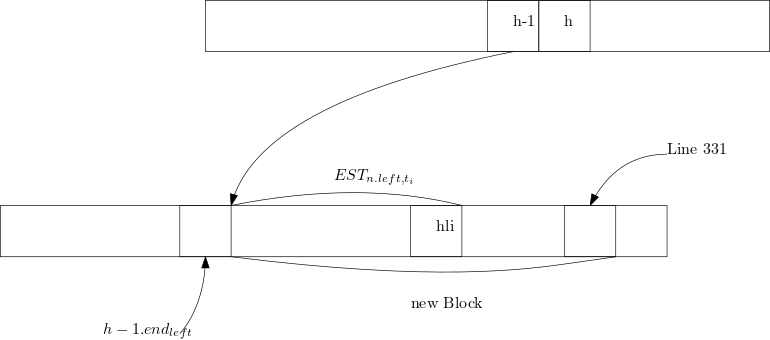
\includegraphics[width=5in]{pics/trueRefresh}
  \caption{New established operations of the left child are in the new block.}
\end{figure}
\begin{lemma}[Stronger True Refresh] \label{lem::prectrueRefresh}
  Let $t_i$ be the time an instance of \nf{n.Refresh()} read the head (Line \ref{readHead}) and $t_t$ be the time its \nf{TryAppend(new, s)} terminates with  and returns \nf{true} (Line \ref{cas}). We have \nf{ops(EST\sub{n.left, t\sub{i}})} $\cup$ \nf{ops(EST\sub{n.right, t\sub{i}})} $\subseteq$ \nf{ops(n.blocks)}.
\end{lemma}
\begin{definition}
  An instance of \nf{Refresh()} is successful iff its \nf{TryAppend(new, s)} terminates with  and returns \nf{true}.
\end{definition}
%\it{Mention this new block is establish in t\sub{t}. last sentece is not complete}

%\begin{lemma}[falseRefresh] \label{lem:falseRefresh}
%    If instance \nf{r} of \nf{n.Refresh()} reads value \nf{s} on line \ref{readHead} and then returns \nf{false}, then there is another instance $r^\prime$ of \nf{n.Refresh()} that has performed a successful \nf{TryAppend(new, s)}. A \nf{TryAppend()} is successful if its \nf{CAS} is successful.
%\end{lemma}
%\begin{proof}
%  If there is no other concurrent successful \nf{n.Refresh()} then \nf{n.Refresh()} would succeed in Line 313. So there is another \nf{n.Refresh()}, that has appended its block in \nf{n.blocks[h]} after Line 310 of the first \nf{n.Refresh()}. 
%%Otherwise the other \nf{Refresh(n)} should have read \nf{h$^\prime$>h} instead of \nf{h} for \nf{n.head}(Line 52).
%\end{proof}

\pagebreak

\begin{definition}
Let $_{R_1}t$ be the time $R_1$ is invoked and $t_{R_2}$ be the time $R_2$ terminates.
  $_{line}t$ is the immediate time before running Line $line$.   $t_{line}$ is the immediate time after running Line $line$. $_{line}t^{op}$ is the immediate time before running Line $line$ of operation $op$.   $t_{line}^{op}$ is the immediate time after running Line $line$ of operation $op$.
\end{definition} 

\begin{lemma}[Double Refresh] \label{doubleRefresh}
  Consider two consecutive instances $R_1$, $R_2$ of \nf{Refresh()} on internal node \nf{n} by a process $p$. If $R_1$ and $R_2$ both fail and return false, then we have \nf{ops(EST\sub{n.left, \sub{R1}t})} $\cup$ \nf{ops(EST\sub{n.right, \sub{R1}t})} $\subseteq$ \nf{ops(EST\sub{n, t\sub{R2}})}.
\end{lemma}
\begin{proof}
  

If $R_2$ reads some value greater than $i+1$ in Line \ref{readHead} it means a successful instance of \nf{Refresh()} performed its Line \ref{readHead} after $t_{\ref{readHead}}^{R_1}$ and finished its Line \ref{incrementHead1} or \ref{incrementHead2} before $t_{\ref{readHead}}^{R_2}$, from Lemma~\ref{lem::prectrueRefresh} by the end of this instance \nf{ops(EST\sub{n.left, t\sub{1}})} $\cup$ \nf{ops(EST\sub{n.right, t\sub{1}})} has been propagated.

 Let $R_1$ read $i$ and $R_2$ read $i+1$ from Line \ref{readHead}. As $R_2$'s \nf{TryAppend()} returns \nf{false}, there is another successful instance $R_2^\prime$ of \nf{n.Refresh()} that has done \nf{TryAppend()} successfully into \nf{n.blocks[i+1]} before $R_2$ tries to append. Since $R_2^\prime$ creates the block after reading the value $i+1$ from \nf{n.head} (Line \ref{readHead}) and $R_1$ reads the value $i$ from \nf{n.head} and the \nf{head}'s value is increasing by Lemma \ref{lem::headProgress} then $t_{R2^\prime \; \ref{readHead}} > t_{R1 \; \ref{readHead}} > _{R_1}t$ (see Figure \ref{fig::doubleRefresh}). By Lemma \ref{lem::prectrueRefresh} after $R_2^\prime$'s \nf{CAS} ($t_{\ref{cas}}^{R_2^\prime}$) we have \nf{ops(EST\sub{n.left, t\sub{1}})} $\cup$ \nf{ops(EST\sub{n.right, t\sub{1}})} $\subseteq$ \nf{ops(n.blocks)}. Also by Lemma \ref{lem::headInc} on $R_2$ the value  of \nf{n.head}  head is more than $i+1$ after $R_2^\prime$ terminates, so the block appended by $R_2^\prime$ to \nf{n} is established by then ($\nf{n.head}\geq i+2 > i+1$). To summarize, $_{R_1}t$ is before $R_2^\prime$'s read of \nf{n.head} ($t_{\ref{readHead}}^{R_2^\prime}$) and $R_2^\prime$'s successful \nf{CAS} is before $R_2$'s termination. So, by Lemma \ref{lem::prectrueRefresh}, \nf{ops(EST\sub{n.left, t\sub{1}})} $\cup$ \nf{ops(EST\sub{n.right, t\sub{1}})} $\subseteq$ \nf{ops(EST\sub{n, t\sub{2}})}.
%It is obvious that the \nf{new} constructed by the second Refresh in Line 36 contains the blocks in \nf{new} by $R_1$ which $R_1^\prime$ did not contain, since \nf{n.head} is only increasing (Maybe Lemma~\ref{lem::oldnewOrder}). If $R_2$ succeeds by Lemma~\ref{lem::trueRefresh} the claim holds. If not, it is deduced that \nf{n.blocks[h]} was not \nf{null} before $R_2$'s \nf{CAS}. Furthermore, \nf{n.blocks[h]} was \nf{null} before reading \nf{h} by $R_1$. So there is a successful \nf{Refresh()} after the read of \nf{h} in $R_1$ and before the \nf{CAS} of $R_2$. This \nf{Refresh()} contains all the new established operations before Line 35 (Maybe Lemma~\ref{lem::oldnewOrder}) and by Lemma~\ref{lem::trueRefresh} our claim holds. See Figure~\ref{}.
\end{proof}

\begin{figure}[hbt]
  \center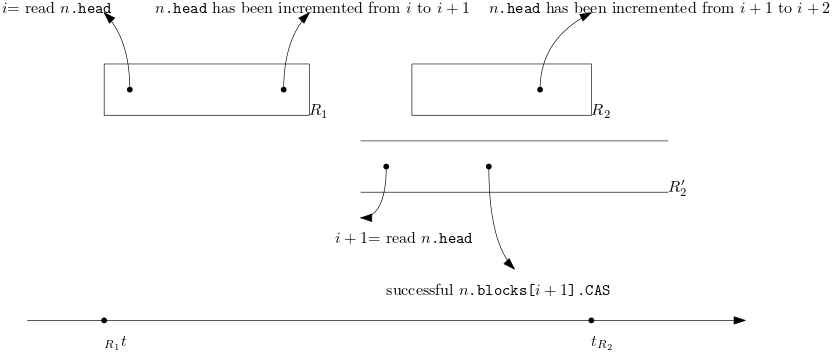
\includegraphics[width=6in]{pics/compactdouble.png}
  \caption{\label{fig::doubleRefresh}$_{R_1}t<$ $t_{\ref{readHead}}^{R_1}$ $<$ incrementing \nf{n.head} from $i$ to $i+1$ $<$ $t_{\ref{readHead}}^{R_2^\prime}$ $<$ $t_{\ref{cas}}^{R_2^\prime}$ $<$ incrementing \nf{n.head} from $i+1$ to $i+2$ $<t_{R_2}$} 
\end{figure}


%  Block \nf{new} is created of new established subblocks of children of \nf{n}(Lemma \ref{lem::createBlock}, Line 46). If \nf{CAS} in Line 48 succeeds then by Lemma~\ref{lem::trueRefresh} new established blocks will be in \nf{n}.
 

\begin{corollary}
  \nf{ops(EST\sub{n.left, \sub{\ref{firstRefresh}}t})} $\cup$ \nf{ops(EST\sub{n.right, \sub{\ref{firstRefresh}}t})} $\subseteq$ \nf{ops(EST\sub{n, t\sub{\ref{secondRefresh}})}}
\end{corollary}
\begin{proof}
  If the first \nf{Refresh()} in line \ref{firstRefresh} returns \nf{true} then by Lemma \ref{lem::trueRefresh} the claim holds. Also if first \nf{Refresh()} failed and the second \nf{Refresh()} succeeded the claim still holds by Lemma \ref{lem::trueRefresh}. Finally, if both failed the claim is satisfied by Lemma \ref{doubleRefresh}.
\end{proof}

\pagebreak


\begin{corollary}[Propagate Step] \label{doublyRefresh}
All operations in \nf{n}'s children's established blocks before running line \ref{firstRefresh}  of a \nf{Propagate} routine are guaranteed to be in \nf{n}'s established blocks after line~\ref{secondRefresh}.
\end{corollary}
\begin{proof}
If \ref{firstRefresh} or \ref{secondRefresh} succeed, the claim is true by Lemma \ref{lem::trueRefresh}. Otherwise Lines \ref{firstRefresh} and \ref{secondRefresh} satisfy the preconditions of Lemma \ref{doubleRefresh}.
\end{proof}

\begin{corollary}\label{lem::appendExactlyOnce}
  After \nf{Append(blk)} finishes \nf{ops(blk)}$\subseteq$\nf{ops(root.blocks[x])} for exactly one \nf{x}.
\end{corollary}
\begin{proof}
After \nf{Append(blk)}'s termination, \nf{blk} is in \nf{root.blocks} since \nf{blk} is established  in the leaf it has been added to. By applying Lemma \ref{doublyRefresh} inductively it is propagated up to the root. Finally Lemma \ref{append} shows  only one block in the root contains \nf{blk}.
\end{proof}


\begin{lemma}[Block Size Upper Bound]\label{blockSize}
Each block contains at most one operation of each processs.
\end{lemma}
\begin{proof}
To derive a contradiction, assume there are two operations $op_1$ and $op_2$ of process $p$ in block $b$ in node $n$. Without loss of generality $op_1$ is invoked earlier than $op_2$. A process cannot invoke more than one operations concurrently, so $op_1$ has to be finished before $op_2$. By Corollary \ref{lem::appendExactlyOnce}, before appending $op_2$ to the tree $op_1$ exists in every node on the path from $p$'s leaf to the root, because $op_1$'s \nf{Append} is finished before $op_2$'s \nf{Append} starts. So, there is some block $b^\prime$  before $b$ in $n$ containing $op_1$.  Existence of $op_1$ in $b$ and $b^\prime$ contradicts Lemma \ref{append}.
\end{proof}

\begin{lemma}[Subblocks Upperbound]\label{subBlocksBound}
Each block has at most $p$ direct subblocks.
\end{lemma}
\begin{proof}
The claim follows directly from Lemma \ref{blockSize} and the observation that each block appended to the tree contains at least one operation, due to the test on Line~\ref{addOP}. We can also see the blocks in the leaves have exactly one operation in the \nf{Enqueue()} and \nf{Dequeue()} routines.
\end{proof}


\pagebreak

\begin{lemma}[Get correctness] \label{get}
If $\nf{n.blocks[b].num\sub{enq}} \geq \nf{i}$ then \nf{n.GetENQ(b,i)} returns the \nf{element} enqueued by $E_i(n,b)$.
\end{lemma}
\begin{proof}
We are going to prove this lemma by induction on the height of node \nf{n}. For the base case, \nf{n} is a leaf. Leaf blocks each contain exactly one operation, so by the hypothesis, only \nf{n.GetENQ(b,1)} can be called and only when \nf{n.blocks[b]} contains an enqueue. At Line \ref{getBaseCase}, \nf{n.GetENQ(b,1)} returns the \nf{element} of the \nf{enqueue} operation stored in the $b$th block of leaf \nf{n} .

For the induction step we prove \nf{n.GetENQ(b, i)} returns $E_i(n,b)$, assuming \nf{n.child.GetENQ(subblock, i)} returns $E_i(n.child,b)$. We argue that  Line \ref{leftOrRight} correctly decides whether the \nf{i}th enqueue in  \nf{b}th block  of internal node \nf{n} is in the  left child or right child subblocks of \nf{n.blocks[b]}. From Definition  \ref{ordering} of $E(n,b)$ we know enqueue operations in a block are ordered from left to right and since the leaves of the tree are ordered by process id from left to right, thus operations from the left subblocks come before operations from the right subblocks in a block (See Figure \ref{figGet}). Furthermore the \nf{num\sub{enq-left}} field  in \nf{n.blocks[b]} stores the number of \nf{enqueue()} operations from the blocks's subblocks in the left child of \nf{n}. So the $i$th enqueue operation is propagated from the right child if \nf{i} is greater than \nf{b.num\sub{enq-left}}. Otherwise we should search for the $i$th enqueue in the left child. By definition \ref{def::subblock} and \ref{def::ops} we need to search in subblocks of \nf{n.blocks[b]} from the range \texttt{n.left.blocks[n.blocks[i-1].end\textsubscript{left}+1..n.blocks[i].end\textsubscript{left}]} $\cup$ \texttt{n.right.blocks[n.blocks[i-1].end\textsubscript{right}+1..n.blocks[i].end\textsubscript{right}]}.

If the $i$th \nf{enqueue} of \nf{n.blocks[b]} is in the left child it would be $i$th enqueue in \texttt{n.left.blocks[n.blocks[i-1].end\textsubscript{left}+1..n.blocks[i].end\textsubscript{left}]} by Definition \ref{def::subblock}. Also, we know there are $eb=n.blocks[b-1].sum_{enq-left}$ enqueues in the blocks before this range, so $E_i(n,b)$ is $E_{i+eb}(n.left)$ which is $E_{i^\prime}(n.left,b^\prime)$ for some $b^\prime$ and $i^\prime$. We can compute $b^\prime$ and then search for $i+eb$th enqueue in \tt{n.left}, where $i^\prime$ is \tt{i+eb-n.left.blocks[}$b^\prime-1$\tt{].sum\sub{enq}}. The parameters in Line \ref{leftChildGet} are for searching $E_{i+eb}(n.left)$ in \nf{n.left.block} in the expected range of blocks, so this \nf{BSearch} returns the index of the subblock containing $E_i(n,b)$.

Otherwise the enqueue we are looking for is in the right child. Then, there are \nf{n.blocks[b].num\sub{enq-left}} enqueues ahead of it in \nf{n.blocks[b]} but not in \texttt{n.right.blocks[n.blocks[i-1].end\textsubscript{right}+1..n.blocks[i].end\textsubscript{right}]}. So we need to search for \nf{i-n.blocks[b].num\sub{enq-left}+ n.blocks[b-1].sum\sub{enq-right}} (Line \ref{rightChildGet}). Other parameters for the left child are chosen similarly to the way they were chosen for the right child. 


So, in both cases the direct subblock containing $E_i(n,b)$ is computed in Lines \ref{leftChildGet} and \ref{rightChildGet}.
 Finally, \nf{n.child.GetENQ(subblock, i)} is invoked on the subblock containing $E_i(n,b)$ and it returns $E_i(n,b)$ by the hypothesis of the induction.
\end{proof}

\begin{figure}[hbt]  
  \center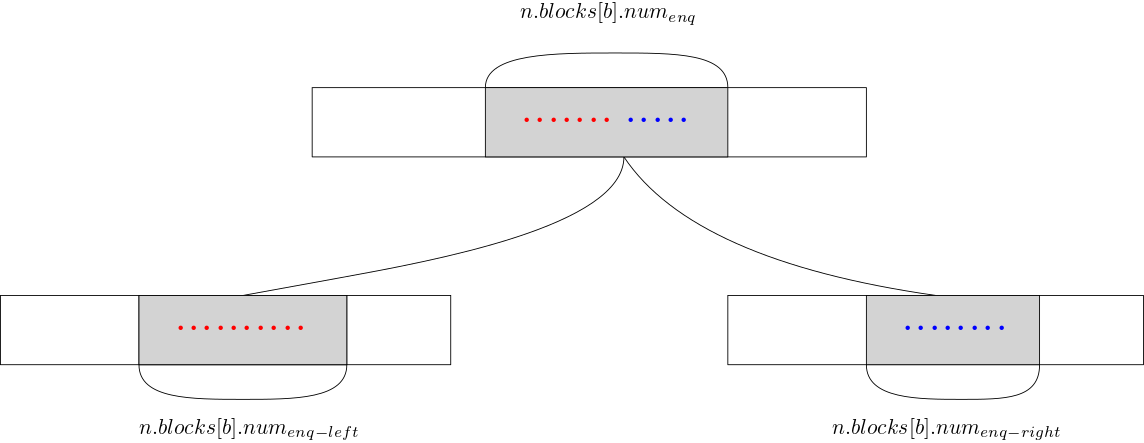
\includegraphics[width=6in]{pics/blockSumEnq.png}
  
  \caption{The number and ordering of the enqueue operations propagated from the left and the right child to \nf{n.blocks[b]}. Enqueue operations from the left subblocks (colored red), are ordered before the enqueue operations from the right child (colored blue).
  }\label{figGet}
\end{figure}

%\textit{I'm not sure it is going to be long and boring to talk about the parameters, since the reader can find out them.}

\pagebreak


\begin{lemma}[DSearch correctness] \label{dsearch}
Assume $\nf{root.blocks[end].sum\sub{enq}}\geq\nf{e}$ and $E_e(root)$'s \nf{element} is the response to some \nf{Dequeue()} operation in \nf{root.blocks[end]}.  \nf{DSearch(e, end)} returns \nf{<b, i>} such that $E_i(root,b)= E_e(root)$.
\end{lemma}
\begin{proof}
It is trivial to see that the doubling search from \nf{root.blocks[end]} to \nf{root.blocks[0]} will find $E_e(root)$ eventually. Because \nf{root.blocks[].sum\sub{enq}} is an increasing value from 0 to some value greater than \nf{e}. So there is a \nf{b} that $\nf{root.blocks[b].sum\sub{enq}}>e$ but $\nf{root.blocks[b-1].sum\sub{enq}}<e$. 

First we show $\nf{end}-\nf{b} \leq 2 \times \big(\nf{root.blocks[b].\size}+\nf{root.blocks[end].\size+1\big)$. From line \ref{addOP}, we know that size of the every block in the tree is greater than 0. So each block in \nf{root.blocks[b..end]} contains at least one \nf{Enqueue} or at least one \nf{Dequeue}. Suppose there were more than \nf{root.blocks[b].\size}\nf{Dequeue}s in \nf{root.blocks[b+1..end-1]}. Then the  queue would become empty at some point after \nf{blocks[b]}'s last operations and before \nf{root.blocks[end]}'s first operation. Which means the response to to a \nf{Dequeue} in \nf{root.blocks[end]} could not be in $E(n,b)$. Furthermore since the size of the queue would become \nf{root.blocks[end].\size} after the \nf{root.blocks[end]}, there cannot be more than \nf{root.blocks[b].\size + root.blocks[end].\size} \nf{Enqueue}s. Because there can be at most \nf{root.blocks[b].\size}\nf{Dequeue}s and the final size is \nf{root.blocks[end].\size}. Overall there can be at most $2 \times$\nf{root.blocks[b].\size+ root.blocks[end].\size} operations in \nf{root.blocks[b+1..end-1]} and since each block size is $\geq 1$ thus there are at most $2 \times$\nf{root.blocks[b].\size+ root.blocks[end].\size} blocks in between \nf{root.blocks[b]} and \nf{root.blocks[end]}. So \nf{end-b}$\leq 2 \times$\nf{root.blocks[b].\size+root.blocks[end].\size+1}. See Figure \ref{fig::doubling}.

Now that we know there are at most \nf{root.blocks[b].\size+root.blocks[end].\size} blocks in between \nf{root.blocks[b]} and \nf{root.blocks[end]} then with doubling search in $\Theta \big(\log($\nf{root.blocks[b].\size+root.blocks[end].\size}$)\big)$ steps we reach \nf{start=c} that the \nf{root.blocks[c].sum\sub{enq}} is less than \nf{e} and \nf{end-c} is not more than $2\times$\nf{root.blocks[b].\size+root.blocks[end].\size}. Beause otherwise, then \nf{(end-c)/2} satisfied the \nf{root.blocks[(end-c)/2].sum\sub{enq}<e}. In line \ref{doubling} the differnece between \nf{end} and \nf{start} is doubled. See Figure \ref{fig::doubling}.

 After computing \nf{b}, the value \nf{i} is computed via the definition of \nf{sum\sub{enq}} in constant time (Line \ref{DSearchComputei}). So the routine non constant part is the binary search which takes $\Theta(\log$\nf{root.blocks[b].\size+root.blocks[end].\size)}$)$ steps from the first paragraph.

\end{proof}
\begin{figure}[hbt]  
  \center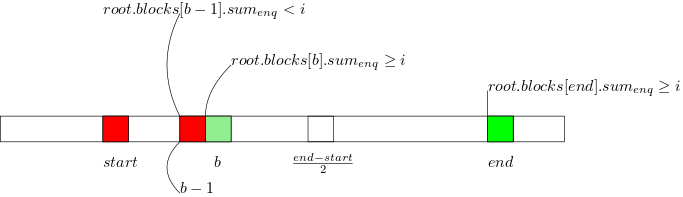
\includegraphics[width=6in]{pics/doubling.png}
  \caption{Distance relations between $b,c,end$}
  \label{fig::doubling}
\end{figure}

%\begin{figure}[hbt]  
%  \center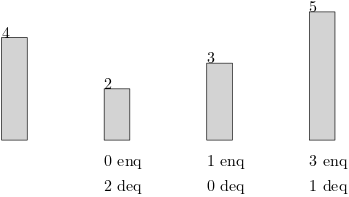
\includegraphics[width=3in]{pics/end-b.png}
%
%  \caption{The number written on top of the bars is the queue size. the first block is $b$ and the last block is $end$.}
%  \label{end-b}
%\end{figure}

\pagebreak

%\begin{definition}
%An enqueue operation is \textit{finished} if its argument is returned by some process. A dequeue operation is \texttt{finished} if it returns \nf{null} or some value. Block \nf{b} is \textit{done} if all operations in \nf{ops(b)} are finished.
%\end{definition}
%\textit{Problem: we increment the \nf{num\sub{finished}} before returning and after the computing response. How to articulate the sentence above in a not confusing correct way?}
%
%\begin{lemma}[help]\label{help}
%After that \nf{TryAppend()} who is helping finishes, prefix for the blocks of \nf{root.blocks[root.FindMostRecentDone]} are done.
%\end{lemma}

\begin{lemma} Let $n.propagates$ be the number of groups of blocks that have been propagated from node \nf{n} to its parent (successful \nf{n.parent.Refresh()}).
We have \nf{num\sub{propagated}}$\leq n.propagates\leq$\nf{num\sub{propagated}+p}. \nf{p} is the number of processes.
\end{lemma}
\begin{proof}
    \tt{num\sub{propagated}} is incremented after propagating (Line \ref{incNP}). Since maybe some process falls sleep before incrementing \tt{num\sub{propagated}} it may be behind by \nf{p}.
\end{proof}


\begin{lemma} \nf{super[]} preserves order from child to parent; i.e. if in node \nf{n} block \nf{b} is before \nf{c} then \nf{b.group} $\leq$ \nf{c.group}
\end{lemma}
\begin{proof} Line \ref{setGroup}. Since  \nf{num\sub{propagated}} is increasing.\end{proof}

\begin{lemma} Let \nf{b, c} be in node \nf{n}, if \nf{b.group} $\leq$ \nf{c.group} then \nf{super[b.group]} $\leq$ \nf{super[c.group]}\end{lemma}
\begin{proof} Line \ref{setSuper}.\end{proof}

\begin{lemma}
The number of the \nf{block}s with \nf{group=i} in a node is $\leq p$.  
\end{lemma}
\begin{proof}For the sake of simplicity we assumed all the blocks are propagated from the left child.
\begin{figure}[hbt]
  \center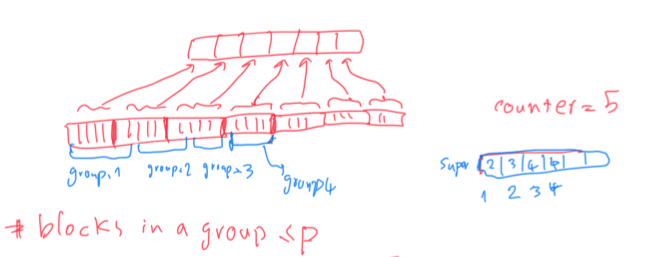
\includegraphics[width=5in]{pics/index1}
\end{figure}  
\end{proof}


% \item In a propagate step at most 2 different time values are read \\ If there are more than 2 numbers then the smallest number should have been propagated far before.
% \item There are at most $p^2$ blocks with same time value in a node. \\ At most p processes could die before line 27 and each contains at most p elements.
\begin{lemma} \nf{super[i+1]-super[i]}$\leq p$\end{lemma}
\begin{proof}
 In a Refresh with successful CAS in line 46, \nf{super} and \nf{counter} are set for each child in lines 48,49. Assume the current value of the counter in node \nf{n} is \nf{i+1} and still \nf{super[i+1]} is not set. If an instance of successful \nf{Refresh(n)} finishes \nf{super[i+1]} is set a new value and a block is added after \nf{n.parent[sup[i]]}. There could be at most $p$ successful unfinished concurrent instances of \nf{Refresh()} that have not reached line 49. So the distance between \nf{super[i+1]} and \nf{super[i]} is less than $p$.
 \begin{figure}[hbt]
  \center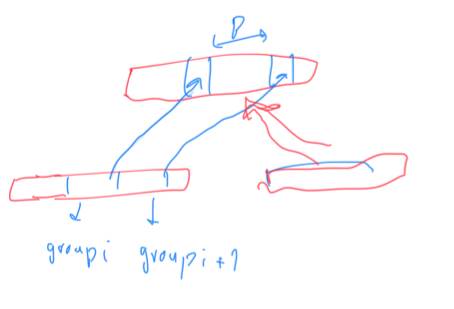
\includegraphics[width=4in]{pics/index2}
\end{figure}  
\end{proof}
\begin{lemma}[super property]\label{superCounter}
If \nf{super[i] $\neq$ null} in node \nf{n}, then \nf{super[i]} is the index of the superblock of a block with \nf{time=i} in \nf{n.parent.blocks}.
\end{lemma}
\begin{lemma}\label{superRange} Superblock of \nf{b} is within range $\pm 2p$ of the \nf{super[b.group]}.
\end{lemma}

\begin{proof} \nf{super[i]} is the index of the superblock of a block containing block b, followed by Lemma \ref{superCounter}. \nf{super(b)} is the real superblock of b. \nf{super(t]} is the index of the superblock of the last block with time \nf{t}. If \nf{b.time} is \nf{t} we have:
$$super[t]-p\leq super[t-1]\leq super(t-1] \leq super(b) \leq super(t+1)\leq super(t+1]\leq super[t]+p$$
\end{proof}

\begin{lemma}
Search in each level of \nf{IndexDeq()} takes $O(\log p)$ steps.  
\end{lemma}
\begin{proof}
Show preconditions are satisfied and the range is $p$.  
\end{proof}

\begin{lemma}[Computing SuperBlock]\label{superBlock}
For the \nf{superblock} value computed in line \ref{computeSuper} of \nf{n.IndexDEQ(b,i)} we have \nf{n.parent.blocks[superblock]} contains $D_{n,b,i}$.
\end{lemma}
\begin{proof}
First we show the value read for \nf{super[b.group]} in line 418 is not null.
  Values \nf{np\textsubscript{dir}} read in lines \ref{setNP}, \nf{super} are set before incrementing in lines \ref{setSuper},\ref{incNP}. So before incrementing \nf{num\sub{propagated}, super[num\sub{propagated}]} is set so it cannot be null while reading. Then by Lemma \ref{superRange}if we search in the range $p$, we can find the superblock.

\end{proof}


\begin{lemma}[Index correctness]
 If $\nf{n.blocks[b].num\sub{deq}}\geq\nf{i}$ then \nf{n.IndexDEQ(b,i)} returns the rank in $D(root)$ of $D_{n,b,i}$.
\end{lemma}
\begin{proof}
We will prove this by induction on the distance of \nf{n} from the \nf{root}. We can see the base case where \nf{n} is root is trivial (Line \ref{indexBaseCase}).
  In the non-root nodes \nf{n.IndexDEQ(b,i)} computes the superblock of the $i$th Dequeue in the $b$th block of \nf{n} in \nf{n.parent} by Lemma \ref{superBlock} (Line \ref{computeSuper}). After that the order in $D(n.parent, superblock)$ is computed. Note that by Lemma \ref{blockSize} in each block there is at most one operation from each process and operations of one type are ordered based on the order in the subblocks (See Figure \ref{fig::orderFromSubblocks}). Finally \nf{index()} is called on \nf{n.parent} recursively and it returns the correct response from induction hypothesis. If the operation was propagated from the right child the number of dequeues from the left child are added to it (Line \ref{considerRight}), because the left child operations come before the right child operations (Definition \ref{ordering}).
\end{proof}
\textit{Make sure to show preconditions of all invocation of \nf{BSearch} are satisfied.}

\begin{figure}[hbt]  
  \center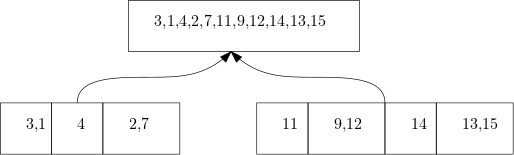
\includegraphics[width=4in]{pics/orderFromSubblocks.png}
  \caption{Relation of ordering of operations of a block from its subblocks}
  \label{fig::orderFromSubblocks}
\end{figure}


\pagebreak



%\begin{lemma}[Search Ranges]\label{search}
%  Preconditions of all invocation of \nf{BSearch} are satisfied.
%\end{lemma}
%\begin{proof}
%  
%Line 83: \nf{Get(i)} is called if the result of a dequeue is not null. The search is among all blocks in the root.
%
%Line 88: This search tries to find the ith enqueue, knowing that it is in the left child. Search is done over the left subblocks. The start and end of the range are followed by definition. Line 92 is the same.
%
%Line 101: Here, the goal is to find the superblock. We know the distance between answer and the \nf{super[i]} is at most $p$, since at most $p$ processes could die.
%
%\end{proof}
\begin{definition}
   Assume the operations in $L$ are applied on an empty queue. If element of \nf{enqueue e} is the response to  \nf{dequeue d} then we say \nf{R(d)=e}. If \nf{d} 's response id \nf{null} (queue is empty) then \nf{R(d)=null}.
\end{definition}

\begin{definition}
In an execution on a queue, the dequeue operations that return some value are called \it{non-null dequeues}.  
\end{definition}
\begin{observation} \label{responseToADeq}
In a sequential execution on a queue, $k$th non-null dequeue returns the \nf{element} of $k$th enqueue.
\end{observation}

\begin{lemma}\label{sizeCorrectness}
  \nf{root.blocks[b].\size}is the \size of the queue if the operations in the prefix for the $b$th block in the root are applied with the order of $L$.  
\end{lemma}
\begin{proof}
 need to say? :: If the \size of a queue is greater than 0 then a \nf{Dequeue()} would decrease the \size of the queue, otherwise the \size of the queue remains 0. By definition \ref{ordering} enqueue operations come before dequeue operations in a block in $L$.

We prove the claim by induction on \nf{b}. Base case \nf{b=0} is trivial since the queue is initialy empty and \nf{root.blocks[0].size=0}. For \nf{b=i} we are going to use the hypothesis for \nf{b=i-1}. If there are more than \nf{root.blocks[i-1].size+ root.blocks[i].sum\sub{enq}} dequeue operations in \nf{root.blocks[i]} then the queue would become empty after \nf{root.blocks[i]}. Otherwise we can compute the size of the queue after $b$th block using with this equality \nf{root.blocks[b].size= root.blocks[b-1].size+ root.blocks[b].sum\sub{enq}- root.blocks[b].sum\sub{deq}} (Line \ref{computeLength}). See Table \ref{qhistory} for an example of running some blocks of operations on an empty queue.
\end{proof}

\begin{lemma}[Duality of \#non-null dequeues and \nf{block.size}] \label{numberOfNND}
If the operations are applied with the order of $L$, the number of non-null dequeues in the prefix for a block \nf{b} is \nf{b.sum\sub{enq}-b.\size}
\end{lemma}
\begin{proof}
There are \nf{b.sum\sub{enq}} enqueue operations in the prefix for \nf{b}, then the size of the queue after the prefix for \nf{b} is \nf{\#enqs - \#non-null dequeues} in the prefix for \nf{b}, by Observation 35. So \nf{\#non-null dequeues} is \nf{b.sum\sub{enq}-b.\size}. The correctness of the \nf{block.\size}field is shown in Lemma \ref{sizeCorrectness}.
\end{proof}

\begin{lemma}\label{nullReturn}
\nf{R(D\sub{root,b,i})} is \nf{null} iff \nf{root.blocks[b-1].\size+ root.blocks[b].num\sub{enq}- i <0}.
\end{lemma}


\begin{lemma}[Computing Response] \label{computeHead}
\nf{FindResponse(b,i)} returns \nf{R(D\sub{root,b,i}).element}.
\end{lemma}
\begin{proof}
First note that by Definition \ref{ordering} the linearization ordering  of operations will not change as new operations come so instead of talking about the linearization of operations before the $E_i(root, b)$ we talk about what if the whole operation in the linearization are applied on a queue.

$D_{root,b,i}$ is $D_{root,root.blocks[b-1].sum_{deq}+i}$ from the definition \ref{ordering} and \it{$sum_{enq}$}.  $D_{root,b,i}$ returns \nf{null} if \nf{root.blocks[b-1].\size+ root.blocks[b].num\sub{enq}- i <0} by Lemma \ref{nullReturn} (Line \ref{checkEmpty}). Otherwise if it is $d^\prime$th non-null dequeue in $L$ it returns $d^\prime$th enqueue by Observation \ref{responseToADeq} . By Lemma \ref{numberOfNND} there are \nf{root.blocks[b-1].sum\sub{enq} - root.blocks[b-1].\size} non-null dequeue operations before prefix for \nf{root.blocks[b-1]}. Note that the dequeues in \nf{root.blocks[b]} before the $i$th dequeue are non-null dequeues. So the response is $E_{i - root.blocks[b-1].size + root.blocks[b-1].sum\sub{deq}}(root)$ (Line \ref{computeE}). See figure \ref{computeResponseDetail}.

After computing \nf{e} we can find \nf{b,i} such that $E_i(root,b)=E_e(root)$ using \nf{DSearch} and then find its \nf{element} using \nf{GetEnq} (Line \ref{findAnswer}).
\end{proof}

\begin{figure}[hbt]  
  \center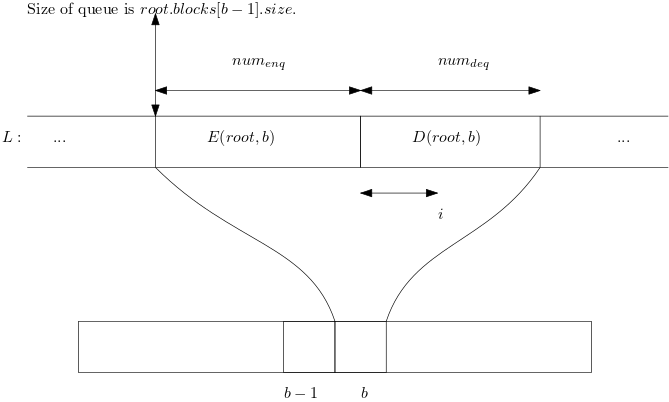
\includegraphics[width=2in]{pics/computeResponseDetail.png}\caption{The position of $E_i(root,b)$.}
\label{computeResponseDetail}
\end{figure}

\begin{table}[hbt]
\centering
  \begin{tabular}{c|c|c|c|c}
    \hline &\texttt{DEQ()} & \texttt{ENQ(5)}, \texttt{ENQ(2)}, \texttt{ENQ(1)}, \texttt{DEQ()}& \texttt{ENQ(3)}, \texttt{DEQ()}&  \texttt{ENQ(4)}, \texttt{DEQ()}, \texttt{DEQ()}, \texttt{DEQ()}, \texttt{DEQ()}\\ \hline
    \#enqueues & 0 & 3 & 1 & 1 \\ \hline
        \#dequeues & 1 & 1 & 1 & 4 \\ \hline
            \#non-null dequeues & 0 & 1 & 2 & 5 \\ \hline
                size & 0 & 2 & 2 & 0 \\ \hline
  \end{tabular}
  \caption{An example of root blocks fields. Blocks are from left to right and operations in the blocks are also from the left to right.}\label{qhistory}
\end{table}


%\begin{proof}
%  \nf{head} is incremented in lines 51, 54 after trying to append a block to the index of the last \nf{head} read. If it was successful, we have to do this, but if it was unsuccessful, it means it has appended to the index before, so we have to update the \nf{head}. If a process dies before line 51, another process will increment \nf{head} in line 54.
%\end{proof} 

\pagebreak

\begin{theorem}[Main]
The queue implementation is linearizable.
\end{theorem}
\begin{proof}
  We choose $L$ in Definition \ref{ordering} to be linearization ordering of operations and prove if we linearize operations as $L$ the queue works consistently.
\end{proof}
%\begin{lemma}
%Operations in a block have a time point in common (There is a time $t$ all the operations are running).
%\end{lemma}

\begin{lemma}[satisfiability]
$L$ can be a linearization ordering.
\end{lemma}
\begin{proof}
To show this we need to say if in an execution, \nf{op\sub{1}} terminates before \nf{op\sub{2}} starts then \nf{op\sub{1}} is linearized before \nf{op\sub{2}}. If \nf{op\sub{1}} terminates before \nf{op\sub{2}} starts it means \nf{op\sub{1}.Append()} is terminated before \nf{op\sub{2}.Append()} starts. From Lemma \ref{append} \nf{op\sub{1}} is in \nf{root.blocks} before \nf{op\sub{2}} propagates so \nf{op\sub{1}} is linearized before \nf{op\sub{2}} by Definition \ref{ordering}.

Once some operations are aggregated in one block they will be propagated together up to the root and we can linearize them in any order among themselves. Furthermore in L we arbitrary choose the order to be by process id, since it makes computations in the blocks faster .
\end{proof}

\begin{lemma}[correctness]
  If operations are applied as $L$ on a sequential queue, the sequence of the responses would be the same as our algorithm.
\end{lemma}

\begin{proof}
\it{Old parts to review}
  We show that the ordering $L$ stored in the root, satisfies the properties of a linearizable ordering.
  \begin{enumerate}
    \item If $op_1$ ends before $op_2$ begins in $E$, then $op_1$ comes before $op_2$ in $T$.\\$\blacktriangleright$ This is followed by Lemma \ref{append}. The time $op_1$ ends it is in root, before $op_2$, by Definition \ref{ordering} $op_1$ is before $op_2$.
    \item Responses to operations in $E$ are same as they would be if done sequentially in order of $L$. \\$\blacktriangleright$ Enqueue operations do not have any response so it does no matter how they are ordered. It remains to prove  Dequeue $d$ returns the correct response according to the linearization order. By Lemma \ref{computeHead} it is deduced that the head of the queue at time of the linearization of $d$ is computed properly. If the Queue is not empty by Lemma \ref{get} we know that the returning response is the computed index element.
  \end{enumerate} 
\end{proof}

\pagebreak


\begin{lemma}[Amortized time analysis]
%  \nf{n.GetEnq(b,i), n.Index(b,i)} take $O(\log^2 p)$ steps. Search in the root may take $O(\log Q+ p^2)$ steps. Helping is done every $p^2$ block appended to the root and takes $p\times \log^2p$ steps. Amortized time consumed for helping by each process is $O(\log^2 p)$.
\nf{Enqueue()} and \nf{Dequeue()}, each take $O(\log^2 p + \log q)$ steps in amortized analysis. Where $p$ is the number of processes and $q$ is the size of the queue at the time of invocation of operation.
\end{lemma}
\begin{proof}
\nf{Enqueue(x)} consists of creating a \nf{block(x)} and appending it to the tree. The first part takes constant time. To propagate \nf{x} to the root the algorithm tries two \nf{Refresh}es in each node of the path from the leaf to the root (Lines \ref{firstRefresh}, \ref{secondRefresh}). We can see from the code  that each \nf{Refresh} takes constant number of steps since creating a block is done in constant time and does $O(1)$ \nf{CAS}es. Since the height of the tree is $\Theta(\log p)$, \nf{Enqueue(x)} takes $O(\log p)$ steps.

A \nf{Dequeue()} creates a block with null value element, appends it to the tree, computes its order among enqueue operations, and returns the response. The first two part is similar to an \nf{Enqueue} operation. To compute the order of a \nf{dqueue} in $D(n)$ there are some constant steps and \nf{IndexDeq()} is called. \nf{IndexDeq} does a search with range $p$ in each level (Lemma \ref{superRange}) which takes $O(log^2 p)$ in the tree. In the \nf{FindResponse()} routine \nf{DSearch()} in the root takes $\Theta(\log$(\nf{root.blocks[b].\size+root.blocks[end].\size}) by Lemma \ref{dsearch}, which is $O(\log$ size of the queue when \nf{enqueue} is invoked$)+\log$ size of the queue when \nf{dequeue} is invoked$)$. Each search in \nf{GetEnq()} takes $O(\log p)$ since there are $\leq p$ subblocks in a block (Lemma \ref{subBlocksBound}), so \nf{GetEnq()} takes $O(\log^2 p)$ steps.

If we split \nf{DSearch} time cost between the corresponding \nf{Enqueue}, \nf{Dequeue}, in amortized we have \nf{Enqueue} takes $O(\log p +q)$ and \nf{Dequeue} takes $O(\log^2 p +q)$ steps.
\end{proof}

\begin{lemma}[CASes invoked]
An \nf{Enqueue()} or \nf{Dequeue()} operation, does at most $4\log p$ \nf{CAS} operations.
\end{lemma}
\begin{proof}
  In each height of the tree at most 2 times \nf{Refresh()} is invoked and  every \nf{Refresh()} has 2 \nf{CAS}es, one in Line \ref{cas} and one in Lines \ref{incrementHead1} or \ref{incrementHead2}.
\end{proof}
\end{document}

